% !TEX root = Zusammenfassung.tex

% Dokumentdefinition, Einstellungen und Packages laden
\documentclass[a4paper,11pt,numbers=noendperiod,bibliography=totocnumbered,listof=totocnumbered,abstracton]{scrreprt}
\usepackage[ngerman]{babel}
\usepackage[utf8]{inputenc} %windows latin1
\usepackage[babel,german=quotes]{csquotes}
\usepackage[T1]{fontenc}
\usepackage{lmodern}% Schrift ist bei allen modernen TeX-Distributionen dabei und der Standard-T1-Schrift deutlich ¸berlegen 
\usepackage{setspace}						% Paket um Absätze zu definieren
\usepackage[left=4cm,right=2cm,top=2.5cm,bottom=2.5cm,includeheadfoot,headheight=1.3\baselineskip]{geometry}% Paket für Seitenlayout

\usepackage{amsmath}						% AMS Pakete für neue Mathe-Umgebungen und -Zeichen
\usepackage{amsfonts}
\usepackage{amssymb}		% Paket f¸r Symbole. ‹bersicht: http://amath.colorado.edu/documentation/LaTeX/Symbols.pdf

\usepackage{blindtext} % Beispieltext

\usepackage{wrapfig} % Bild neben Text
\usepackage{multicol} % Mehrspaltenmodus
\usepackage{subfigure} % Bilder nebeneinander
\usepackage{stmaryrd} % Widerspruch Blitze


\renewcommand{\arraystretch}{1.5} % General space between rows (1 standard)
\setlength{\tabcolsep}{5pt} % General space between cols (6pt standard)

%% Tiefe des Inhaltsverzeichnisses
\setcounter{tocdepth}{3}


%%%%%%%%%%% Seitenzahlen rechts positionieren %%%%%%%%%%%%%%%%%%%
\usepackage{scrpage2}
\pagestyle{scrheadings}
\clearscrheadings
\clearscrplain
\ofoot[\pagemark]{\pagemark}
\cfoot{}
%%%%%%%%%%%%%%%%%%%%%%%%%%%%%%%%%%%%%%%%%%%%%%%%%%%%%%%%%%%%%%%%%

%%%%%%%%%%% Fuflnoten durchlaufend nummerieren %%%%%%%%%%%%%%%%%%%
\usepackage{remreset}
\makeatletter\@removefromreset{footnote}{chapter}\makeatother
%%%%%%%%%%%%%%%%%%%%%%%%%%%%%%%%%%%%%%%%%%%%%%%%%%%%%%%%%%%%%%%%%


%%%%%%%%%%% Abk¸rzungsverzeichnis erstellen %%%%%%%%%%%%%%%%%%%%%
\usepackage[german,intoc]{nomencl}
% Befehl umbenennen in abk
%\let\abk\nomenclature
% Deutsche ‹berschrift
\renewcommand{\nomname}{Abk¸rzungsverzeichnis}
% Punkte zw. Abk¸rzung und Erkl‰rung
\setlength{\nomlabelwidth}{.20\hsize}
\renewcommand{\nomlabel}[1]{#1 \dotfill}
% Zeilenabst‰nde verkleinern
\setlength{\nomitemsep}{-\parsep}
\makenomenclature
%%%%%%%%%%%%%%%%%%%%%%%%%%%%%%%%%%%%%%%%%%%%%%%%%%%%%%%%%%%%%%%%%

\usepackage{titleref} % um auf Titel (‹berschriften) zu referenzieren
\usepackage{hyperref} % Links auf Inhaltsverzeichnis und Verweise verteilen...
\usepackage{url} % f¸r \url{http://www}, Option hyp erlaubt auch Umbruch nach "-"

%%%%%%%%%%%%%%%%%%%%%%%%%%%%%%%%%
% The following is needed in order to make the code compatible
% with both latex/dvips and pdflatex.
\ifx\pdftexversion\undefined
\usepackage[dvips]{graphicx}
\else
\usepackage[pdftex]{graphicx}
\DeclareGraphicsRule{*}{mps}{*}{}
\fi
%%%%%%%%%%%%%%%%%%%%%%%%%%%%%%%%%

%%TABELLEN
\usepackage{booktabs}

\onehalfspacing % Anderthalbzeilig
\setlength{\parskip}{10pt plus 4pt minus 2pt}
\parindent0pt

% COMMANDS
\newcommand{\homo}{Homomorphismus }
\newcommand{\homos}{Homomorphismen }
\newcommand{\epi}{Epimorphismus }
\newcommand{\epis}{Epimorphismen }
\newcommand{\mono}{Monomorphismus }
\newcommand{\monos}{Monomorphismen }
\newcommand{\syssig}{$Sys(\Sigma)$ } 
\newcommand{\prop}{Proposition }
\newcommand{\defi}{Definition }
\newcommand{\coro}{Corollary }
\newcommand{\lem}{Lemma }

%



% BEGINN HAUPTDOKUMENT
\begin{document}

\pagestyle{scrheadings}

% Titelseite
%\include{includes/titelseite}

% Seitennummerierung für Inhaltsverzeichnis
\pagenumbering{Roman}
\setcounter{page}{1}
% Inhaltsverzeichnis
\tableofcontents 
\newpage

% Abkürzungsverzeichnis
%\printnomenclature

% Seitennummerierung für Hauptteil setzen
\setcounter{chapter}{0}
\setcounter{secnumdepth}{2}
\pagenumbering{arabic}
\setcounter{page}{1} 



\chapter{Signaturen, Systeme und Homomorphismen}


\section{Homomorphismus}
\paragraph{Definition 4 (Def)}
Zwei algebraische Systeme mit selber Signatur $\Sigma$ $h: A \rightarrow B$ Familie totaler Abbildungen.

Wenn $f^A$ für $x$ definiert ist, dann muss $f^B$ für $h^w(x)$ definiert sein.
[$f^B(h^w(x)) = h^v(f^A(x))$]

\paragraph{Notation 5 (Hom. als Familie von Abbildungen (\underline{h}))}

\paragraph{Proposition 6 (Identity)}

Die Identität ist ein Homomorphismus. $id: A \rightarrow A$.

\paragraph{Proposition 7 (Komposition)}
Wenn $f: A \rightarrow B$ und $g: B \rightarrow C$ homomorphismen, dann ist $g \circ f$ wieder ein Homomorphismus.

\paragraph{Fact 8 (Eigenschaften von Identitäten und Kompositon)}
Identitäten kürzbar und Klammern 'verschiebbar'  (Assoziativität).

\section{Kategorien}

\paragraph{Definition 9 (Def)}

$C= (O, M, id, \circ)$ [Objects, Morphism-Sets, Identitäten, Kompositionen] \\
Identitäten kürzbar und Klammern 'verschiebbar'  (Assoziativität).

\paragraph{Definition 12 (Kategorien von Mengen \& Abbildungen)}
$C= (O^{Set}, M^{Set}, id^{Set}, \circ^{Set})$ [Die Klasse aller Mengen, die Menge aller Abbildungen, die identitätische Abbildung, Kompositionen von Abbildungen] \\

\paragraph{Definition 13 (Kategorien algebraischer Systeme)}
$Sys(\Sigma)$ ist Kategorie aller $\Sigma$ Systeme und Homomorphismen zwischen diesen. \\
\underline{Sys}($\Sigma$) die Kategorie aller $\Sigma$ Systeme in der alle Operationsnamen als totale Funktionen interpretiert werden und alle Homomorphismen zwischen diesen.

\section{Derived Systems}

\subsection{Subsysteme}

\subsubsection{Subsysteme}
\paragraph{Definition 15 (Def)} 

Schwaches Subsystem ($B \subseteq A$), wenn:
\begin{enumerate}
\item Die Trägermengen in Teilmengenrelation $B_s \subseteq A_s$
\item Wenn Operation im Untersystem definiert ist und y liefert, muss sie auch im "drüber liegenden" System sein und y liefern.
\end{enumerate}

Volles Subsystem $B \subseteq_f A$, wenn schwaches Untersystem und: \\
\begin{enumerate}
\item $f^A(x)=y$ definiert und $x,y \in B_s$ dann $f^B(x)=y$
\end{enumerate}

Geschlossenes Subsystem $B \subseteq_c A$, wenn volles Untersystem und: \\
\begin{enumerate}
\item  $f^A(x)=y$ definiert und $x \in B_s$ dann $y \in B_s$
\end{enumerate}

\paragraph{Proposition 16 (Geschlossene Subsysteme von totalen Systemen)}
Jedes geschlossene Subsystem eines totalen Systems ist total.

\subsubsection{Intersection (Schnitt) und Union (Vereinigung)}

\paragraph{Definition 17 Schnitt}
Sei $\mathfrak{B}=\left(B^{i}\subseteq A\right)_{i\in I}$ ein nicht leere Schnitt.
Der Schnitt $\bigcap\mathfrak{B}$ ist definiert als 
\begin{enumerate}
\item Sortenweiser Schnitt über die Trägermengen ($s\in S$: $\left(\bigcap\mathfrak{B}\right)_{s}=\bigcap_{i\in I}B_{s}^{i}$).
\item Alle Operationen zum sortenweisen Schnitt der Trägermengen ($f\in O$: $f^{\bigcap\mathfrak{B}}=\bigcap_{i\in I}f^{B^{i}}$).
\end{enumerate}

\paragraph{Proposition 18 Eigenschaften der Schnitte von Subsystemen}
\begin{enumerate}
\item $\bigcap\mathfrak{B}$ ist ein algebraisches System. D.h. die Operationen sind wohldefiniert.
\item Der Schnitt ist selber Subsystem von A ($\bigcap\mathfrak{B} \subseteq A$)
\begin{enumerate}
\item \emph{Notiz CT:} Der Schnitt über volle Untersysteme ist wieder voll
\item \emph{Notiz CT:} Der Schnitt über geschlossene Untersysteme ist wieder geschlossen
\end{enumerate}
\item Der Schnitt ist Untersystem jedes $B^i$
\item Für alle Subsysteme $X$ von $B^i$ gilt, dass sie Untersystem von $\bigcap\mathfrak{B}$ sind.
\end{enumerate}

\paragraph{Definition 20 Vereinigung}
Sei $\mathfrak{B}=\left(B^{i}\subseteq A\right)_{i\in I}$ eine nicht leere Vereinigung.
Die Vereinigung $\bigcup\mathfrak{B}$ ist definiert als 
\begin{enumerate}
\item Sortenweise Vereinigung der Trägermengen ($s\in S$: $\left(\bigcup\mathfrak{B}\right)_{s}=\bigcup_{i\in I}B_{s}^{i}$).
\item Alle Operationen zur sortenweisen Vereinigung der Trägermengen ($f\in O$: $f^{\bigcup\mathfrak{B}}=\bigcup_{i\in I}f^{B^{i}}$).
\end{enumerate}

\paragraph{Proposition 21 Eigenschaften der Vereinigungen von Subsystemen}
\begin{enumerate}
\item $\bigcup\mathfrak{B}$ ist ein algebraisches System. D.h. die Operationen sind wohldefiniert.
\item Die Vereinigung ist selber Subsystem von A ($\bigcup\mathfrak{B} \subseteq A$)
\item $B^i$ ist Untersystem der Vereinigung ($\bigcup\mathfrak{B}$) [Unterschied zum Schnitt!]
\item Für alle Obersysteme $X$ von $B^i$ gilt, dass $\bigcup\mathfrak{B}$ Untersystem von $X$ ist [Unterschied zum Schnitt!].
\end{enumerate}

\subsubsection{Verband}

\paragraph{Proposition 23 Verband von Subsystemen}
Die Menge von (i) allen (schwachen), (ii) allen vollen und (iii) allen geschlossenen Untersystemen ist ein kompletter Verband bis auf Inklusion.

\subsubsection{Abschluss Operatoren (Closure Operators) \& leere Systeme}

\paragraph{Collorary 24 Abschluss Operatoren}
$B = (B_s \subseteq A_s)_{s \in S}$, dann gibt es ein kleinstes volles ($\left\lceil B\right\rceil _{s}^{f}$) und kleinstes geschlossene ($\left\lceil B\right\rceil _{s}^{c}$) Subsystem, dass B enthält.

\paragraph{Definition 25 Leeres System}
Das leere System $\mathcal{I}$ besteht nur aus leeren Komponenten.

\paragraph{Proposition 26 Leeres System als Untersystem}
\begin{enumerate}
\item $\mathcal{I}$ ist immer das kleinste Subsystem
\item $\left\lceil \mathcal{I}\right\rceil ^{f}$ ist das kleinste volle Subsystem
\item $\left\lceil \mathcal{I}\right\rceil ^{c}$ ist das kleinste geschlossene Subsystem
\end{enumerate}

\paragraph{Proposition 27 Eigenschaften von Abschluss Operatoren}
$x \in \{c,f\}$
\begin{enumerate}
\item $B\subseteq\left\lceil B\right\rceil ^{x}$
\item $B\subseteq B'\implies\left\lceil B\right\rceil ^{x}\subseteq\left\lceil B'\right\rceil ^{x}$
\item $\left\lceil \left\lceil B\right\rceil ^{x}\right\rceil ^{x}=\left\lceil B\right\rceil ^{x}$
\end{enumerate}

\paragraph{Proposition 28 Endlich generierte Systeme}
A ist endlich erzeugt, wenn $A = \left \rceil G \right \rceil^c$ für eine endlich generierte Familie von Mengen $G = (G_s \subseteq A_s)_{s \in S}$

\subsubsection{Inklusions-Homomorphismus}

\paragraph{Proposition 29 Inklusions-Homomorphismus}
$A\subseteq B$, der Inklusions-Morphismus \\ $\subseteq:A\rightarrow B$  ist definiert
für $a\in A_{s}$ durch  $\subseteq(a)=a$

Das Bild eines beliebigen Homorphismus $h: A \rightarrow B$ ist ein Untersystem von $B$.

\subsubsection{Homomorphe Bilder}

\paragraph{Definition 30 Bild eines Homomorphismus}
Trägermengen und Operationen werden abgebildet.

\paragraph{Proposition 31 Bild eines Homomorphismus}
Das Bild eines Homomorphismus ist ein Untersystem.

\paragraph{Proposition 32 Bilder von Kompositionen}
$h:A\rightarrow B$ and $k:B\rightarrow C$ \,
$k\circ h(A)\subseteq k(B)$

\paragraph{Definition 33 Volle und geschlossene Homomorphismen}
$h:A\rightarrow B$ ist voll bzw. geschlossen wenn das Bild $(h(A))$ ein volles bzw. geschlossenes Untersystem der Co-Domain $B$ ist: $h(A) \subseteq^x B$ \, $x \in \{f,c\}$

Jeder volle Homomorphismus von einem totalen System $A$ in ein System $B$ ist geschlossen.

\paragraph{Definition 35 Konstruktion von Abschlüssen}
Sei $A$
System und $\left(B_{s}\subseteq A_{s}\right)_{s\in S}$ Familie von Teilmengen auf den Trägermengen. 
Die Operatoren sind dazu da, um ein Untersystem geschlossen/voll zu machen.
Wir definieren
\begin{enumerate}
\item Konstanten dazu: $\left\lceil B\right\rceil ^{0}=B\cup\left(\left\{ y\in A_{s}\,::\, f^{A}(*)=(p,y,q),\, f\in O_{\epsilon,v}\right\} \right)_{s\in S}$
\item Notwendige Funktionswerte: \\ $\left\lceil B\right\rceil ^{i+1} =\left(\left\lceil B\right\rceil _{s}^{i}\cup\left\{ y\in A_{s}\,::\, f^{A}(x)=(p,y,q),\, f\in O_{w,v},\, x\in\left(\left\lceil B\right\rceil ^{i}\right)^{w},\,|w|\geq1\right\} \right)_{s\in S}$
\item 1 und 2 zusammen: $\left\lceil B\right\rceil ^{*}=\bigcup_{i\in\mathbb{N}_{0}}\left\lceil B\right\rceil ^{i}$
\item Macht es voll:  $\widehat{B}=\left(B,\,\left(f^{A}\cap\left(B^{w}\times B^{v}\right)\right)_{f\in O_{w,v}}\right)$
\item Macht es geschlossen (3 und 4 zusammen):  $\widetilde{B}=\widehat{\left\lceil B\right\rceil ^{*}}$
\end{enumerate}

\paragraph{Proposition 36 Konstruktion von Abschlüssen}

$\left\lceil B\right\rceil ^{f}=\widehat{B}$
und \textup{$\left\lceil B\right\rceil ^{c}=\widetilde{B}$}
\newpage

\paragraph{Lemma 37 Abschlüsse und Homomorphismen}
$h: A \rightarrow C$ und $B_s \subseteq A_s$ Familie von Teilmengen der Trägermengen von A. Dann gilt: $h(\left \lceil B \right \rceil^c) \subseteq \left \lceil \underline{h}(B) \right \rceil^c$

\begin{figure}[h]
\noindent \centering{}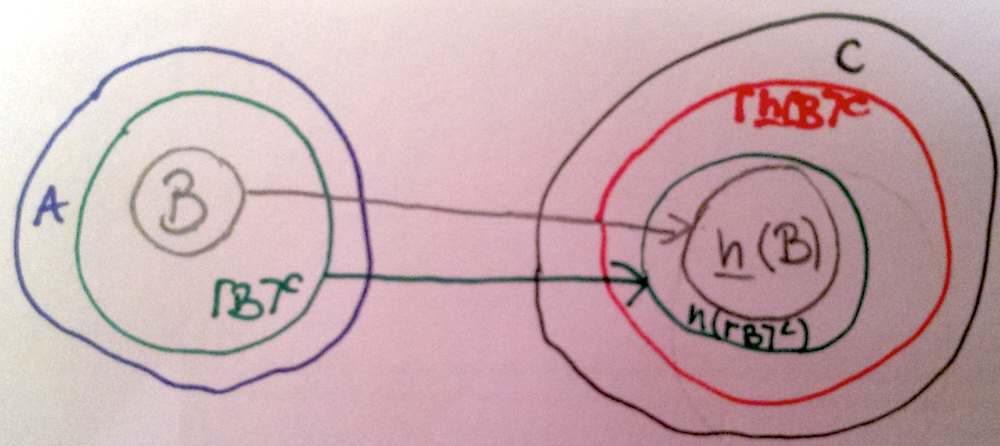
\includegraphics[scale=0.08]{Abbildungen/37}\caption{Abschlüsse und Homomorphismen}
\end{figure}

\subsection{Quotient}

\subsubsection{Kongruenz}

\paragraph{Definition 38 Kongruenzrelation}
Äquirel \&: 
$
x\equiv^{w}x',\, f^{A}(x)=y, f^{A}(x')=y' \, \Rightarrow  \, y\equiv^{v}y'
$

\paragraph{Proposition 39 Schnitt von Kongruenzen}
$\left(\equiv_{i}\right)_{i\in I}$ auf A: $\bigcap_{i\in I}\equiv^{i}$ ist Kongruenz auf A.

\subsubsection{Verband}

\paragraph{Corollary 40 Verband von Kongruenzen}
Die Menge $\mathfrak{C}^{A}=\{\equiv\,::\,\equiv\textrm{ist Kongruenz auf }A\}$
von Kongruenzrelationen auf einem algebraischen System $A$ ist ein vollständiger Verband bis auf Inklusion.

\subsubsection{Abschluss Operator}

\paragraph{Corollary 41 Abschluss Operator}
Kleinste Kongruenz $\left\lceil r\right\rceil _{A}$ auf
$A$ die $r$ enthält.

\subsubsection{Kernel}

\paragraph{Definition 42 Kern eines Homomorphismus}
Kern $h^\equiv$ beinhaltet all die Elemente, die durch den Homomorphismus $h$ auf das Gleiche abgebildet werden.
$h_{s}^{\equiv}=\{(a_{1},a_{2})\,::\, h_{s}(a_{1})=h_{s}(a_{2})\}$

\paragraph{Proposition 43 Kern}
$h^\equiv$ ist eine Kongruenz auf der $h$-Domain.

\paragraph{Proposition 44 Kern einer Komposition}
$m^\equiv \subseteq (n \circ m)^\equiv$ 


\subsubsection{Quotient}

\paragraph{Definition 45 Quotient}
Gegeben System $A$ und $\equiv$ auf A. Der Quotient $A_\equiv$ 
\begin{enumerate}
\item Kongruente Elemente der Trägermenge in eine Äquivalenzklasse schmeissen.
\item $f^{A_{|\equiv}}([x]^{w})=[y]^{v},\,\textrm{wenn }f^{A}(x)=y$
\end{enumerate}

\paragraph{Proposition 46 Quotient von totalen Systemen}
Jeder Quotient eines totalen Systems ist total.

\subsubsection{Natürlicher Homomorphismus}

\paragraph{Proposition 47 Natürlicher Homomorphismus}
Bildet Elemente der Trägermengen in ihre jeweilige Äquivalenzklasse ab ($\equiv : A \rightarrow A_{|\equiv}$). 

\paragraph{Proposition 48 Natürlicher Homomorphismus}
Jeder natürlicher Homomorphismus ist geschlossen.

\paragraph{Proposition 49 Kongruenz Theorem}
$\equiv^{1}$ und $\equiv^{2}$ sind Kongruenzen auf $A$, sodass $\equiv^{1}\,\subseteq\,\equiv^{2}$, dann gibt es einen Homomorphismus $\equiv^{2-1}:A_{|\equiv^{1}}\rightarrow A_{|\equiv^{2}}$
mit $\equiv^{2-1}\circ\equiv^{1}\,=\,\equiv^{2}$.


\subsubsection{Operatoren auf Relationensfamilien}

\paragraph{Proposition 50 Operatoren auf Relationensfamilien}

\begin{enumerate}
\item Symmetrie
\item Reflexivität
\item $r^1_s = r_s$
\item Rekursiver Verkettung 
\item $r^*$ = Vereinigung von 1 bis 4
\item $c^0(r)_s = r_s$
\item $\textrm{c}^{i+1}(r)_{s}=\textrm{c}^{i}(r)_{s}\cup\left\{ \left(y_{i},y'_{i}\right)::f\in O_{w,psq},i=|p|+1,x\left(\textrm{c}^{i}(r)\right)^{w}x',f^{A}(x)=y,f^{A}(x')=y'\right\}$
\item Vereinigung von 6 und 7
\end{enumerate}


\paragraph{Lemma 51}

\begin{enumerate}
\item $r^*$ ist Familie transitiver Relationen.
\item $c^*(r)$ erfüllt Kongruenzbedingungen (Definition 38)
\end{enumerate}


\paragraph{Lemma 52}
Wenn eine Relation $r\subseteq A\times A$ reflexiv ist
und $r\subseteq s\subseteq A\times A$, dann ist $s$ auch reflexiv.


\paragraph{Lemma 53}
Gegeben symmetrische Relation $r$, dann $c^*(r)$ und $r^*$ auch symmetrisch.


\paragraph{Lemma 54}
Gegeben Relation $r$ auf einem totalen $A$. R erfüllt Kongruenzbedingung (Def 38). Dann erfüllt auch $r^*$ die Kongruenzbedingung.


\paragraph{Proposition 55 Konstruktion der generierten Kongruenz}
$A$ total und $r$, dann $\left\lceil r\right\rceil =\left(c^{*}\left(sym\left(r\cup r^{0}\right)\right)\right)^{*}$.

\section{Mono, Epi und Isomorphismen}

\subsection{Isomorphismus}

\paragraph{Definition 57 Sektion, Retraktion und Isomorphismus}
Morphiums $m: A \rightarrow B$ in einer Kategorie $C$.
\begin{enumerate}
\item$m$ ist Sektion wenn $m^{-1} \circ m = id_A$
\item$m$ ist Retraktion  wenn $m \circ m^{-1}  = id_B$
\item $m$ ist Isomorphismus wenn 1 und 2.
\end{enumerate}

\paragraph{Proposition 58/59 Kompositionen von Sektion/Retraktion}
\begin{enumerate}
\item $n, m$ Sektionen/Retraktionen $\Rightarrow$ $n \circ m$ Sektion/Retraktion.
\item $n \circ m$ Sektion/Retraktion $\Rightarrow$ m ist Sektion/ n ist Retraktion.
\end{enumerate}

\paragraph{Proposition 60 Eigenschaften von Isomorphismen}
\begin{enumerate}
\item Alle Identitäten sind Isomorphismen
\item $m$ Isomorphismus $\Rightarrow m^{-1}$ Isomorphismus.
\item $n, m$ Isomorphismen $\Rightarrow n \circ m$ Isomorphismus.
\item $n \circ m$ Isomorphismus und (m Retraktion oder n Sektion) $\Rightarrow $ m und n Isomorphismen.
\item Isomorphismus $i: a \rightarrow b \Rightarrow a \approx b$ ist eine Äquivalenz.
\end{enumerate}

\paragraph{Proposition 61 Isomorphismus in Set}
Kategorie Set, Map $f: a \rightarrow b$
\begin{enumerate}
\item $f$ ist Sektion, wenn $f$ injektiv ist und $a \neq \emptyset$
\item $f$ ist Retraktion, wenn $f$ surjektiv 
\item $f$ ist Isomorphismus, wenn $f$ bijektiv
\end{enumerate}

\paragraph{Proposition 62 Notwendige Bedingungen für Isomorphismen in $Sys(\Sigma)$}
$h: A \rightarrow B$ ist Isomorphismus in $Sys(\Sigma) \Rightarrow$
\begin{enumerate}
\item $h$ ist injektiv in allen Komponenten
\item $h$ ist surjektiv in allen Komponenten
\item $h$ ist voll
\end{enumerate}
 
\paragraph{Proposition 63 Hinreichende Bedingungen für Isomorphismen in $Sys(\Sigma)$}
Wenn $h$ bijektiv (Prop 62: 1 und 2) und voll (Prop 62: 3) ist, dann ist es ein Isomorphismus.

\paragraph{Corollar 64 Ismomorphismus $Sys(\Sigma)$ und $\underline{Sys}(\Sigma)$ }
\begin{enumerate}
\item Die Isomorphismen in $Sys(\Sigma)$ sind bijektive und volle Homomorphismen.
\item Die Isomorphismen in $\underline{Sys}(\Sigma)$ sind bijektive Homomorphismen.
\end{enumerate}

\subsection{Generelle Mono- und Epimorphismen}

\begin{multicols}{2}{}
\columnseprule1pt

\textbf{\underline{Monomorphismus}}

\textbf{Definition 65 (Def)} \\
$m \circ p = m \circ q \Rightarrow p = q$

\textbf{Proposition 66} \\
Jede Sektion ist monisch.

\textbf{Proposition 67 (Komposition)} \\
(1) $n,m$ monic $\Rightarrow n \circ m$ monic. \\
(2) $n \circ m$ monic $\Rightarrow m$ monic.
\\

\textbf{Proposition 68 (Geschlossen unter Iso)} \\
$m: a \rightarrow b$ ist monisch, $a \approx a'$, $b \approx b'$ $\Rightarrow \approx \circ \, m \, \circ \approx: a' \rightarrow b'$ ist mono. 

\textbf{Definition 69 (Abstraktes Subobjekt)} \\
Abstraktes Subobjekt ($a,m:a\rightarrowtail b$) eines Objektes $b$ in Kategorie $C$ \\ - ist ein Objekt $a \in C$ \\ - zusammen mit einem Mono $m:a\rightarrowtail b$

Zwei Subobjekte \\ - $(a_{1},\, m_{1}:a_{1}\rightarrowtail b)$ \\
- $(a_{2},\, m_{2}:a_{2}\rightarrowtail b)$  \\ 
des selben Objektes $b$ sind die selben abstrakten Subobjekte wenn es einen Iso $\approx:a_{1}\rightarrow a_{2}$ gibt, so dass $m_{1}=m_{2}\,\circ\approx$.


\columnbreak
\textbf{\underline{Epimorphismus}}

\textbf{Definition 73 (Def)} \\
$p \circ e = q \circ e \Rightarrow p = q$

\textbf{Proposition 74 } \\
Jede Retraktion ist episch.

\textbf{Proposition 75 (Komposition)} \\
(1) $n,m$ epic $\Rightarrow n \circ m$ epic. \\
(2) $n \circ m$ epic $\Rightarrow n$ epic.\\



\textbf{Proposition 76 (Epi ist abstr. 'notion')} \\
$m: a \rightarrow b$ ist episch, $a \approx a'$, $b \approx b'$ $\Rightarrow \approx \circ \, m \, \circ \approx: a' \rightarrow b'$ ist episch. 

\textbf{Definition 77 (Abstrakter Quotient)} \\
Abstrakter Quotient ($b,e: a \twoheadrightarrow b$)  eines Objektes $a$ in Kategorie $C$ \\ - ist ein Objekt $b \in C$ \\ - zusammen mit einem Epi $e:a \twoheadrightarrow b$

Zwei Quotienten \\ - $(b_{1},\, e_{1}:a \twoheadrightarrow b_1)$ \\
- $(b_{2},\, e_{2}:a \twoheadrightarrow b_2)$  \\ 
des selben Objektes $a$ sind die selben abstrakten Quotienten, wenn es einen Iso $\approx:b_{1}\rightarrow b_{2}$ gibt, so dass $ \approx \circ \, e_{1}=e_{2} $.


\end{multicols}
\newpage

\begin{multicols}{2}
\columnseprule1pt

\textbf{\underline{Monomorphismus}} \\

\textbf{Proposition 70 (Monische Retraktion)} \\
Eine monische Retraktion ist ein Isomorphismus.

\textbf{Proposition 71 (Mono in Set)} \\
Hom. in $Set$ ist monisch $\Leftrightarrow$  er injektiv ist. \\
\\
\\
\\
\\
\\

\textbf{Proposition 72 (Mono in $Sys(\Sigma)$)} \\
Hom. in $Sys(\Sigma)$ ist monisch $\Leftrightarrow$  er injektiv in allen Komponenten ist.
\\
\\

\columnbreak
\textbf{\underline{Epimorphismus}}

\textbf{Proposition 78 (Epische Sektionen)} \\
Eine epische Sektion ist ein Isomorphismus

\textbf{Proposition 79 (Epi in Set)} \\
Hom. in $Set$ ist episch $\Leftrightarrow$ er surjektiv ist.

\textbf{Proposition 80 (Hinreichende Bedingungen für Epis in $Sys(\Sigma)$)} \\
Jeder surjektive Homomorphismus in $Sys(\Sigma)$ ist episch.

\textbf{Proposition 82 (Epi in $Sys(\Sigma))$)} \\
Hom. in $Sys(\Sigma)$ ist episch $\Leftrightarrow$  das kleinste, geschlossene Subsystem von $B$ induziert durch das Bild von $h$ übereinstimmt mit $B$, das heißt: $\underbrace{\left\lceil h(A)\right\rceil ^{C}}_{Def. 35} =B$ .

\end{multicols}

\subsection{Spezielle Mono- und Epimorphismen}

\begin{multicols}{2}{}
\columnseprule1pt

\textbf{\underline{Extremale Monomorphismus}}

\textbf{Definition 83 (Extremaler Mono)} \\
Mono $m: a \rightarrow b$ ist extremal, wenn für jede Zerlegung $m = f \circ e$
gilt: ist $e$ episch dann ist $e$ auch Iso.

\textbf{Proposition 84 } \\
Jede Sektion ist ein extremaler Mono.

\textbf{Proposition 85 (Komposition)} \\
$n \circ m$ extremal Mono $\Rightarrow m$ extremal Mono.


\columnbreak
\textbf{\underline{Extremale Epimorphismus}}

\textbf{Definition 89 (Extremale Epis)} \\
Epi $e: a \rightarrow b$ ist extremal, wenn für jede Zerlegung $e = m \circ f$
gilt: ist $m$ monisch dann muss $m$ auch Iso sein.

\textbf{Proposition 90 } \\
Jede Retraktion ist ein extremaler Epi.

\textbf{Proposition 91 (Komposition)} \\
$e \circ f$ extremal Epi $\Rightarrow e$ extremal Epi.


\end{multicols}

\newpage

%
\begin{multicols}{2}{}
\columnseprule1pt

\textbf{\underline{Extremale Monomorphismus}}

\textbf{Proposition 86 (Extr. Mon. ist abstr. 'Notion') } \\
$m: a \rightarrow b$ ist extremaler Mono, $a' \approx a$, $b \approx b'$ $\Rightarrow \approx \circ \, m \, \circ \approx$ ist extremaler Mono. 
\\
\\
Notiz: Jeder Mono in $Set$ ist extremal.
\\
\\
\\
\\
\textbf{Proposition 87 (Extr. Mono in $Sys(\Sigma)$) } \\
Hom. in $Sys(\Sigma)$ ist extremaler Mono $\Leftrightarrow$  er injektiv und geschlossen.


\columnbreak
\textbf{\underline{Extremale Epimorphismus}}


\textbf{Proposition 92 (Extr. Epi ist abstr. 'Notion') } \\
$e: a \rightarrow b$ ist extremaler Epi, $a' \approx a$, $b \approx b'$ $\Rightarrow \approx \circ \, e \, \circ \approx$ ist extremaler Epi. 
\\
\\
Notiz: Jeder Epi ist $Set$ ist extremal. Extremale Epis sind ein geeignetes Modell zur Abstraktion von Quotienten in $Sys(\Sigma)$

\textbf{Proposition 93 (Extr. Epi in $Sys(\Sigma)$) } \\
Hom. in $Sys(\Sigma)$ ist extremaler Epi  $\Leftrightarrow$  er surjektiv und voll.
\end{multicols}


\subsection{Faktorisierungssysteme}

\subsubsection{Faktorisierungssysteme}

\paragraph{\defi 95 Faktorisierungssystem}
$\mathcal{E}$ und $\mathcal{M}$ sind Klassen von Morphismen in $C$.
$(\mathcal{E}$ und $\mathcal{M})$ ist ein Faktorisierungssystem, wenn
\begin{enumerate}
\item Jeder Morphismus $p$ lässt sich in $p = m \circ e$ zerlegen.
\item $\mathcal{E}$ und $\mathcal{M}$ sind geschlossen unter Komposition mit Isomorphie
\item Wenn $m \circ p \, = \, q \circ e$, dann gibt es einen eindeutigen Morphismus $d$ (Diagonale), so dass $m \circ d = q$ und $d \circ e = p$ (siehe \ref{fig:diagonale}).
\end{enumerate}

\begin{figure}[h]
\label{fig:diagonale}
\noindent \centering{}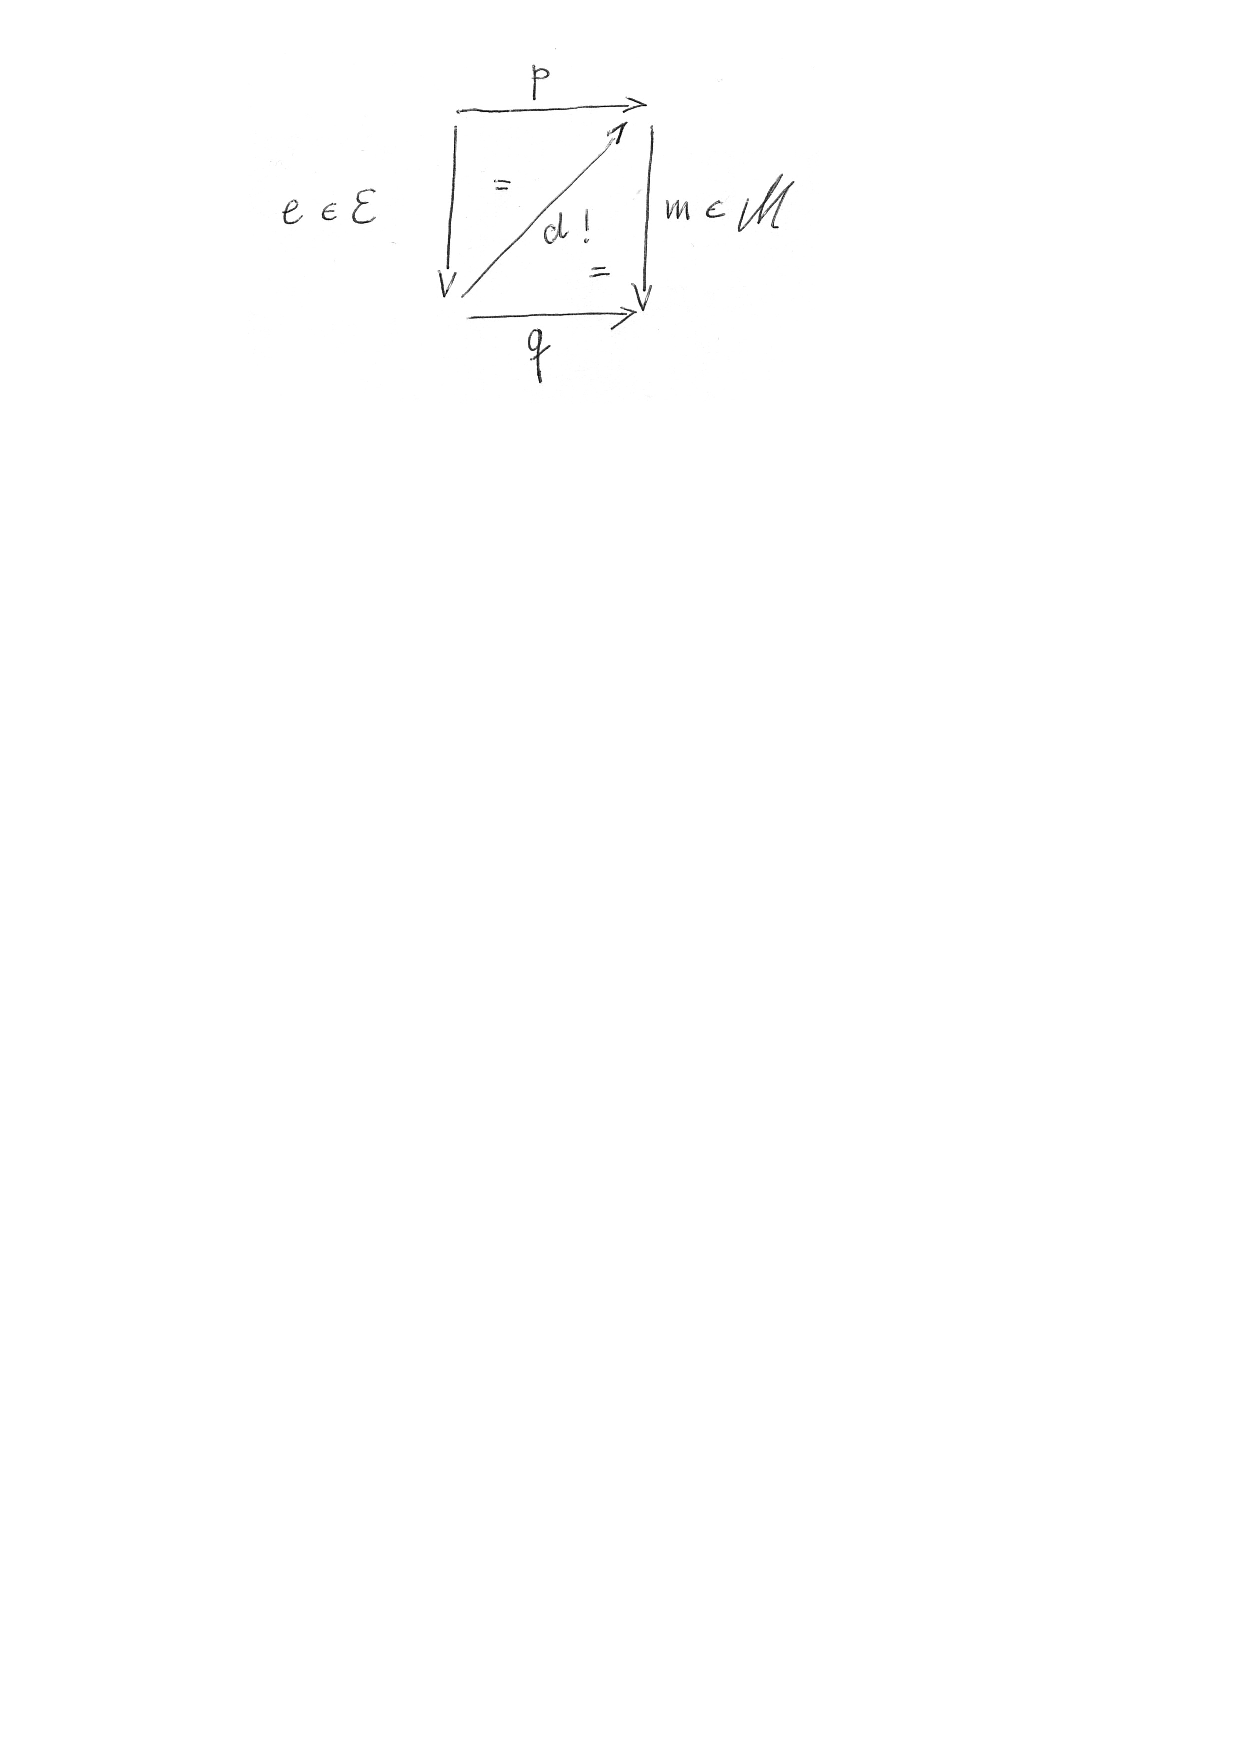
\includegraphics[scale=0.5]{Abbildungen/Diagonal}\caption{Diagonale}
\end{figure}

\paragraph{\prop 96 Eindeutige Faktorisierung}
Faktorisierungen sind eindeutig bis auf Isomorphie:

\begin{enumerate}
\item $(e_{1}:a\rightarrow c_{1},m_{1}:c_{1}\rightarrow b), \\ (e_{2}:a\rightarrow c_{2},m_{2}:c_{2}\rightarrow b)$ sind zwei Faktorisierungen für den selben Morphismus \\ $p:a\rightarrow b$,
\, \, d.h. $m_{1}\circ e_{1}=p=m_{2}\circ e_{2}$ \\
$\Rightarrow$ es gibt Iso $i:c_{1}\rightarrow c_{2}$ mit $i\circ e_{1}=e_{2}$
und $m_{2}\circ i=m_{1}$.
\item $(e:a\rightarrow c,m:c\rightarrow b)$
ist Faktorisierung für $p:a\rightarrow b$ und $i:c\rightarrow d$
ist ein Isomorphismus $\Rightarrow $ $(i\circ e:a\rightarrow d,m\circ i{}^{-1}:d\rightarrow b)$
ist auch Faktorisierung für $p:a\rightarrow b$
\end{enumerate}

\begin{figure}[h]
\label{fig:eindeutig_diagonale}
\noindent \centering{}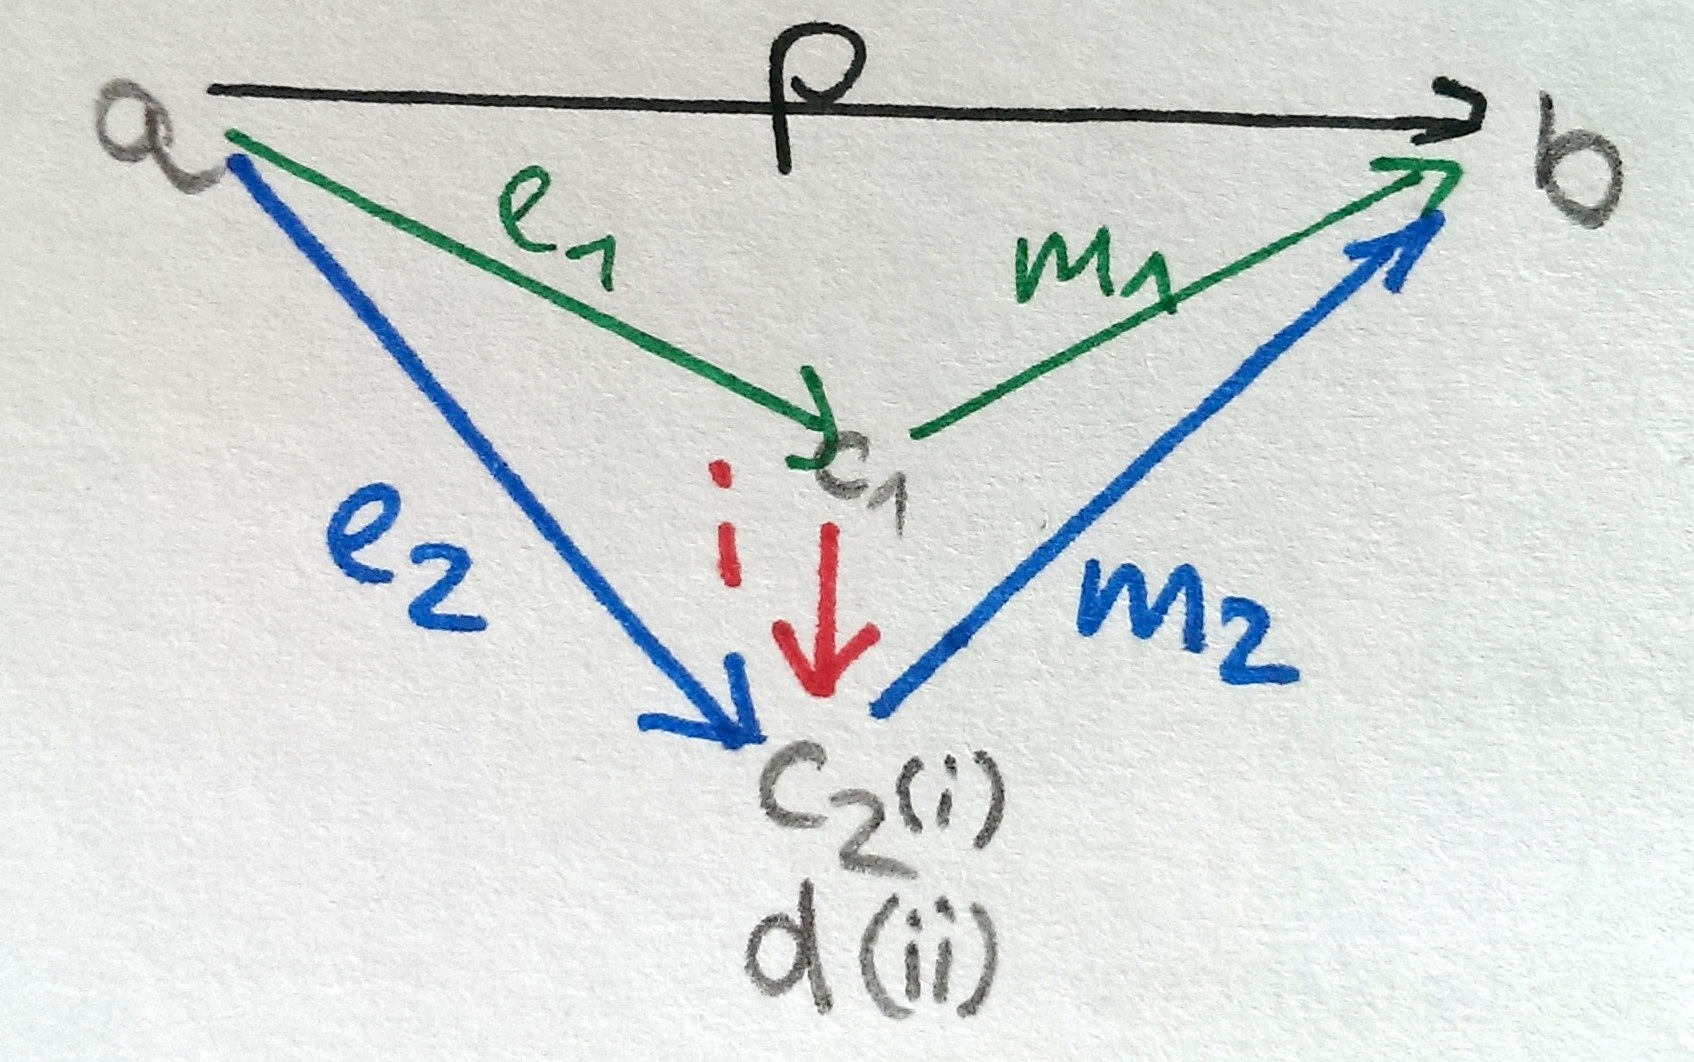
\includegraphics[scale=0.1]{Abbildungen/eindeutig_diagonale}\caption{Eindeutige Diagonale}
\end{figure}

\paragraph{\prop 96 Komposition}
Wenn $(\mathcal{E},\mathcal{M})$ ein Faktorisierungssystem ist, dann sind die Klassen $\mathcal{E}$ und $\mathcal{M}$ geschlossen unter Komposition.

\paragraph{\prop 97 Epi-/Mono-Faktorisierung in Set}
In Set:  $\mathcal{E}$  \epis und $\mathcal{M}$ \monos

\subsubsection{Homomorphismus Theoreme}


\begin{multicols}{2}
\columnseprule1pt

\textbf{\underline{Theorem 1}} 

\textbf{Theorem 99 Homom Theorem 1} \\
$h: A \rightarrow B$ surjektiv und voller Hom. und $k: A \rightarrow C$ ist Hom. so dass $h^\equiv \subseteq k^\equiv$, d.h.
der Kern von $k$ beinhaltet den Kern von $h$ \\ $\Rightarrow$ es gibt einen eindeutigen Homom. \\ $k^*: B \rightarrow C$ so dass $k^* \circ h = k$. \\
$\equiv^h \, \, \, = \, \, \,\equiv^k \, \,\Rightarrow k^*$ ist injektiv.


\columnbreak
\textbf{\underline{Theorem 2}} 

\textbf{Theorem 103 Homom Theorem 2} \\
$h: A \rightarrow B$ injektiver Homom. und \\ $k: C \rightarrow B$ ist Hom. so dass $k(C) \subseteq h(A)$ \\ \\ $\Rightarrow$ es  gibt einen eindeutigen Homom. \\ $k^*: C \rightarrow A$ mit $h\circ k^* = k$ \\
$\left\lceil k(C)\right\rceil ^{c}=h(A)$, then $k^{*} \Rightarrow$ $k^*$ ist epi.

\end{multicols}

\newpage 

\begin{multicols}{2}
\columnseprule1pt

\textbf{\underline{Theorem 1}} \\

\textbf{\lem 100 Invarianter Kern} \\
$m$ injektiver Homom. $\Rightarrow \, \, \equiv^{m \circ h} \, \, = \, \, \equiv^h$ für alle Hom, die mit $m$ komponiert werden können.

\textbf{\coro 101 Extremal epische Faktorisierungen in \syssig} \\
$(\mathcal{E}^{x}, \mathcal{M})$ ist ein Faktorisierungssystem wobei $\mathcal{E}^{x}$ extremaler Epi und $\mathcal{M}$ \mono

\textbf{\coro 102 Komposition extremaler Epis} \\
$e_1 : A \rightarrow B$, $e_2 : B \rightarrow C$ sind zwei extremale Epis in \syssig $\Rightarrow \, e_2 \circ e_1$ ist extremaler Epi.

\columnbreak
\textbf{\underline{Theorem 2}}

\textbf{\lem 104 Invariante Sub-Trägermengen} \\
$e: A \rightarrow B$ epi $\Rightarrow \left\lceil h(B) \right\rceil ^{c} = \left\lceil h\circ e(A)\right\rceil ^{c}$ für alle \homos $h: B \rightarrow C$.

\textbf{\coro 105 Extremal mono Faktorisierungen in \syssig} \\
$(\mathcal{E}, \mathcal{M}^{x})$ ist ein Faktorisierungssystem wobei $\mathcal{E}$ Epi und $\mathcal{M}^{x}$ extremaler \mono

\textbf{\coro 106 Komposition extremaler Monos} \\
$m_1 : A \rightarrow B$, $m_2 : B \rightarrow C$ sind zwei extr. Monos in \syssig $\Rightarrow \, m_2 \circ m_1$ ist extr. Mono.
\end{multicols}

\subsubsection{Surjektive / volle injektive Homomorphismen}

\paragraph{\prop 107 Surjektive und volle injektive Homos}
Konzept der surjektiven und Konzept der vollen inkjektiven Homos ist abstrakt. D.h. Homo $h:A \rightarrow B$ surjektiv/voll und injektiv und $A \approx A'$ und $B \approx B'$ $\Rightarrow \approx \, \, \circ \, \, m \, \, \circ \approx$ ist surjektiv/voll und injektiv.

\paragraph{\coro 109 Surjektive / voll injektive Faktorisierung in \syssig}
($\mathcal{S}$, $\mathcal{FI}$) Faktorisierungssystem in \syssig wobei $\mathcal{S}$ die Klasse aller surjektiven und $\mathcal{FI}$ aller vollen injektiven Morphismen ist.

\newpage


\section{System Komposition}

\subsubsection{Parallele Komposition \& Variante Systeme}


\begin{multicols}{2}
\columnseprule1pt

\textbf{\underline{Parallele Komposition}} 

\textbf{\defi 110 Parallele Komposition} \\
Eine parallele Komposition $A\times B$  \\
(i) $\forall \, s \in S:\,\left(A\times B\right)_{s}=A_{s}\times B_{s}$ \\
(ii) $\forall \, f\in O_{w,v},\, x\in\left(A\times B\right)^{w}:$\\$f^{A\times B}(x)=(y_{A}\times_{v}y_{B})$\\ wenn $f^{A}(x_{A})=y_{A}\textrm{ \emph{und} }f^{B}(x_{B})=y_{B}$\\
Notiz: Parallele Komposition zweier totaler Systeme ist total.

\textbf{\prop 111 Eigenschaften paralleler Komposition} \\
$A,B,C$ sind Systeme $\Rightarrow$ folgende parallele Kompositionen sind Isomorph \\
(1) $A \times B \approx B \times A$ (Kommutiativ)\\
(2) $A \times (B \times C) \approx (A \times B) \times C$ (Assoziativ) \\
(3) $A \times \mathcal{I} \approx \mathcal{I}$ ($\mathcal{I}$ eine Art null-system)


\textbf{\defi 112 Projektionen} \\
$A \times B \Rightarrow$  die Projektionen \\ 
$\left(p_{s}^{A}:\left(A\times B\right)_{s}\rightarrow A_{s}\right)_{s\in S}$
und \\ $\left(p_{s}^{B}:\left(A\times B\right)_{s}\rightarrow B_{s}\right)_{s\in S}$
sind def. durch: Für $x\in\left(A\times B\right)_{s}$: \\(1)
$p_{s}^{A}(x)=x_{A}$ und \\(2) $p_{s}^{B}(x)=x_{B}$

\textbf{\prop 113 Projektionen} \\
Die Projektionen $p^A$ und $p^B$ sind Homoms.

\textbf{\prop 114 Eindeutige Homomorphismen in parall. Kompositionen} \\
$h,k: C \rightarrow (A \times B)$ \homos mit \\
(1) $p_A \circ h \, = \, p_A \circ k$ und 
(2) $p_B \circ h \, = \, p_B \circ k$\\$ \Rightarrow h = k$

\columnbreak
\textbf{\underline{Variante Systeme}} 


\textbf{\defi 115 Variante Systeme} \\
Eine variantes System $A  + B$  \\
(i) $\forall s \in S: \left(A + B\right)_{s}= \left(A_{s}\uplus B_{s}\right)_{|\equiv^{\mathcal{I}}}$ \\ ($\equiv^{\mathcal{I}}$ siehe Skript Seite 28)\\
(ii) $\forall \, f\in O_{w,v},\, [x] \in\left(A + B\right)^{w}:$\\$f^{A + B}[x]= \begin{cases}
\left[y_{A}\right] & \textrm{wenn \ensuremath{x\in A^{w}\textrm{ \emph{und} }}}f^{A}(x)=y_{A}\\
\left[y_{B}\right] & \textrm{wenn \ensuremath{x\in B^{w}\textrm{ \emph{und} }}}f^{B}(x)=y_{B}
\end{cases}$
Notiz: Variantes System zweier totaler Systeme muss nicht total sein.



\textbf{\prop 116 Eigenschaften varianter Systeme} \\
$A,B,C$ sind Systeme $\Rightarrow$ folgende variante Systeme sind Isomorph \\
(1) $A + B \approx B + A$ (Kommutiativ)\\
(2) $A + (B + C) \approx (A + B) + C$ (Assoziativ) \\
(3) $A + \mathcal{I} \approx A$ ($\mathcal{I}$ eine Art neutrales System)


\textbf{\defi 117 Einbettungen} \\
$A + B \Rightarrow$  die Einbettungen \\ 
$\left(i_{s}^{A}:A_{s}\rightarrow\left(A+B\right)_{s}\right)_{s\in S}$
und \\ $\left(i_{s}^{B}:B_{s}\rightarrow\left(A+B\right)_{s}\right)_{s\in S}$
sind def. durch: \\ (1) Für $x\in A_{s}$: $i_{s}^{A}(x)=[x]$ und \\ (2) Für $x\in B_{s}$: $i_{s}^{B}(x)=[x]$.

\textbf{\prop 118 Einbettungen} \\
Die Einbettungen $i^A$ und $i^B$ sind Homoms.

\textbf{\coro 119 Injektive Einbettungen} \\
Signatur ohne Konstanten $\Rightarrow$ Einbettungen: injektiv und geschlossen.

\textbf{\prop 120 Eindeutige Homomorphismen aus varianten Systemen} \\
$h,k: (A+B) \rightarrow C$ \homos mit \\
(1) $h \circ i_A \, = \, k \circ i_A$ und 
(2) $h \circ i_B \, = \, k \circ i_B$\\$ \Rightarrow h = k$
\end{multicols}

\section{Produkte \& Co-Produkte}

\begin{multicols}{2}
\columnseprule1pt

\textbf{\underline{Produkte}} 

\textbf{\defi 121 Produkt} \\
$\mathcal{A}=\left(a_{i}\right)_{i\in I}$, 
$\Pi\mathcal{A}=\left(\Pi\mathcal{A},\left(p_{i}:\Pi\mathcal{A}\rightarrow a_{i}\right)_{i\in I}\right)$: \\
$\forall$ Objekte $c$ und ($x_i : c \rightarrow a_i$) gibt es eindeutig $u: c \rightarrow \Pi \mathcal{A}$
so dass $p_i \circ u = x_i$. \\ $u$ auch genannt $\left\langle x_{i}\right\rangle _{i\in I}$.\\ Das Produkt ist endlich wenn $I$ endlich. 
Siehe Abbildung \ref{fig:121}

\textbf{\prop 122 Produkt ist abstrakt} \\
(1) $\Pi_1 \mathcal{A}$ und $ \Pi_2 \mathcal{A} \Rightarrow \, \, \, \approx: \Pi_1\mathcal{A} \rightarrow \Pi_2\mathcal{A}$, \\ so dass ($p^2_i \circ \approx = p^1_i)_{i\in I}$ \\
(2) $\Pi \mathcal{A}$ und $ \approx : q \rightarrow \Pi \mathcal{A} \, \Rightarrow$\\$ (q, (p_i \circ \approx : q \rightarrow a_i)_{i \in I})$ ist Produkt von $\mathcal{A}$ 


\columnbreak

\textbf{\underline{Co-Produkte}} 

\textbf{\defi 137 Co-Produkt} \\
$\mathcal{A}=\left(a_{i}\right)_{i\in I}$, 
$\sum\mathcal{A}=\left(\sum\mathcal{A}, \left(in_{i}:a_i \rightarrow \sum\mathcal{A} \right)_{i\in I}\right)$: \\
$\forall$ Objekte $c$ und ($x_i : a_i \rightarrow c$) gibt es eindeutig $u: \sum \mathcal{A} \rightarrow c$
so dass $u \circ in_i = x_i$. \\ $u$ auch genannt $\{ x_{i} \} _{i\in I}$.\\ Das Co-Produkt ist endlich wenn $I$ endlich. 
Siehe Abbildung \ref{fig:137}.

\textbf{\prop 138 Abstr Co-Produkt} \\
(1) $\sum_1 \mathcal{A} $ und $ \sum_2 \mathcal{A} \Rightarrow \, \, \, \approx: \sum_1\mathcal{A} \rightarrow \sum_2\mathcal{A}$, \\ so dass ($\approx \circ in^1_i = in^2_i)_{i\in I}$ \\
(2) $\sum \mathcal{A} $ und $ \approx : \sum \mathcal{A} \rightarrow q \, \Rightarrow$\\$ (q, ( \approx \circ in_i : a_i \rightarrow q)_{i \in I})$ is Co-Produkt v. $\mathcal{A}$ 


\end{multicols}

\begin{figure}[h]
\centering
\subfigure[Produkt\label{fig:121}]{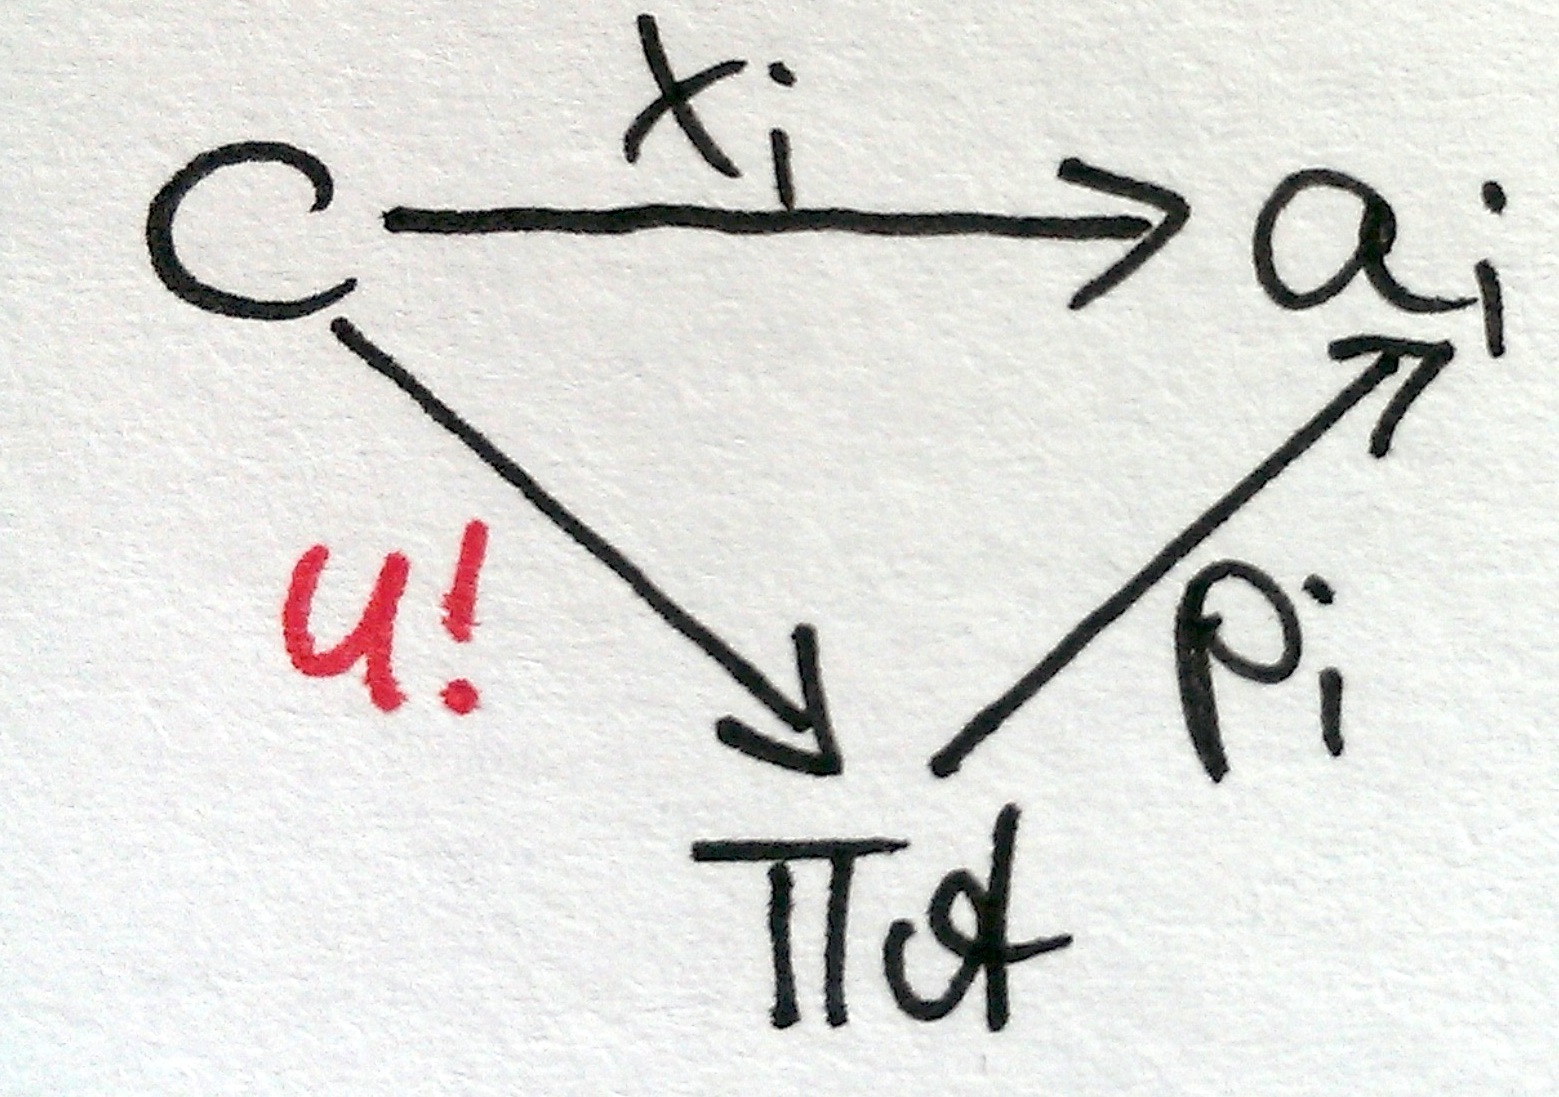
\includegraphics[width=0.21\textwidth]{Abbildungen/121}} \qquad \qquad \qquad
\subfigure[Co-Produkt\label{fig:137}]{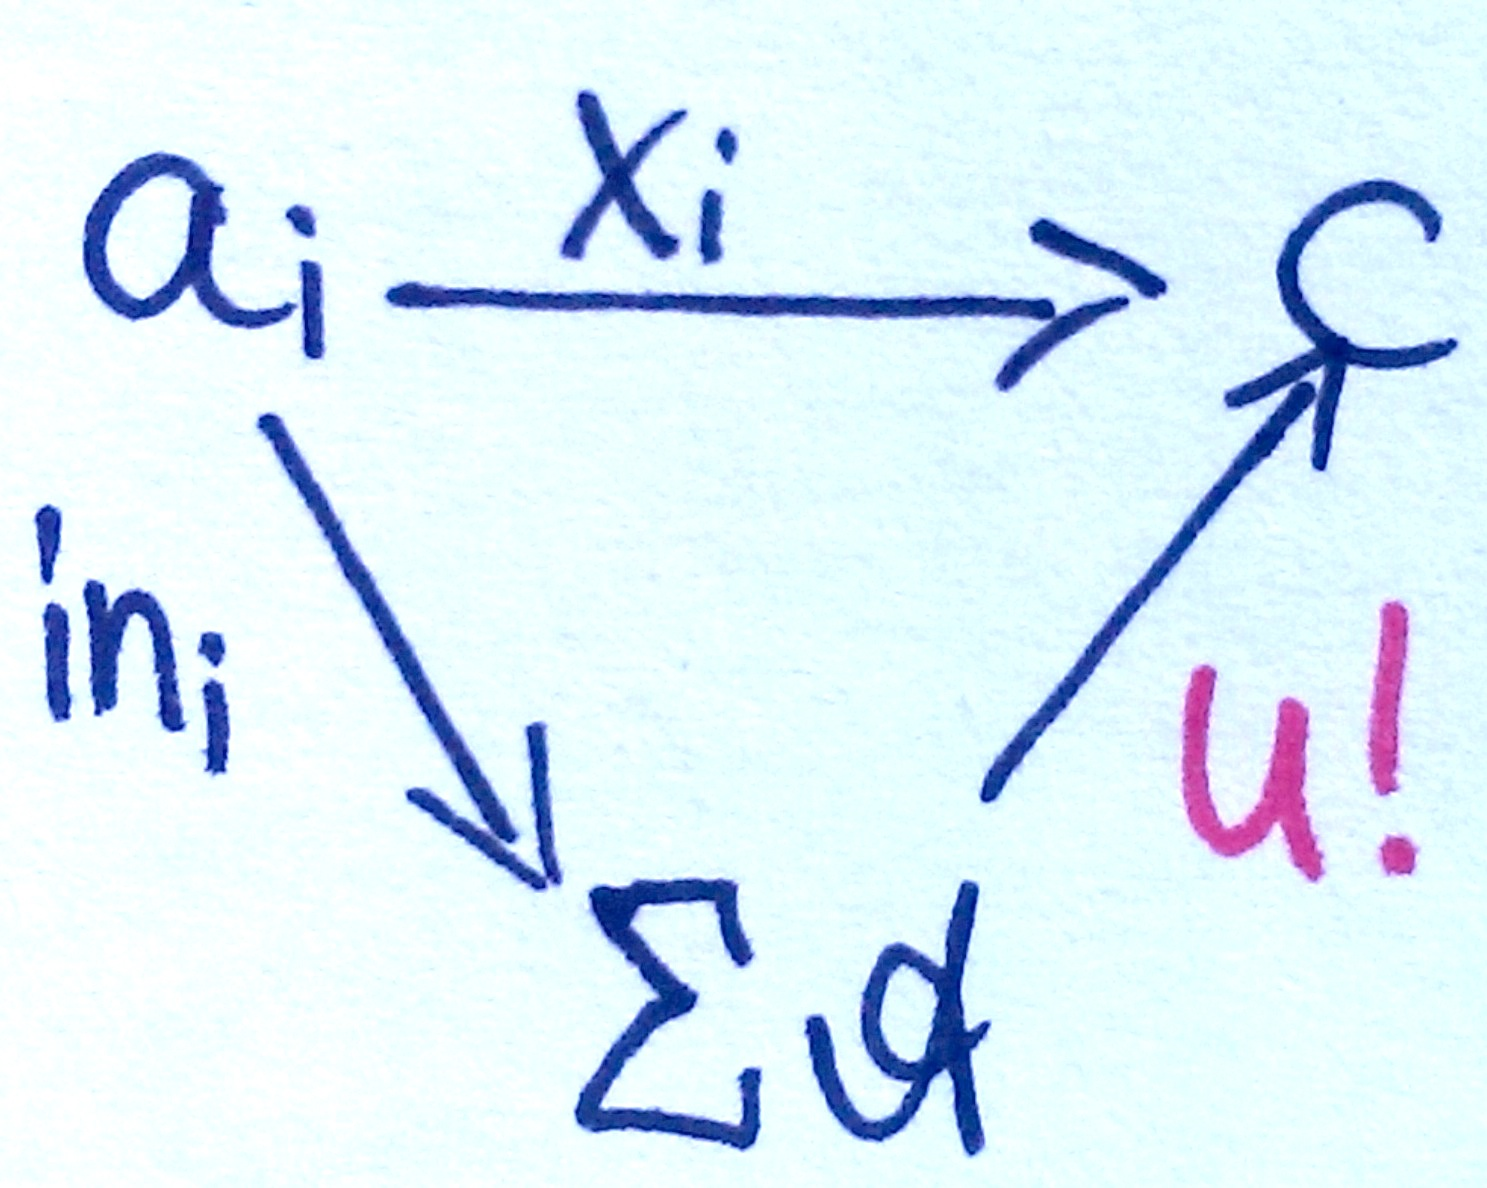
\includegraphics[width=0.18\textwidth]{Abbildungen/137}}
\caption{Definitionen}
\end{figure}

\begin{figure}[h]
\centering
\subfigure[Produkt\label{fig:122}]{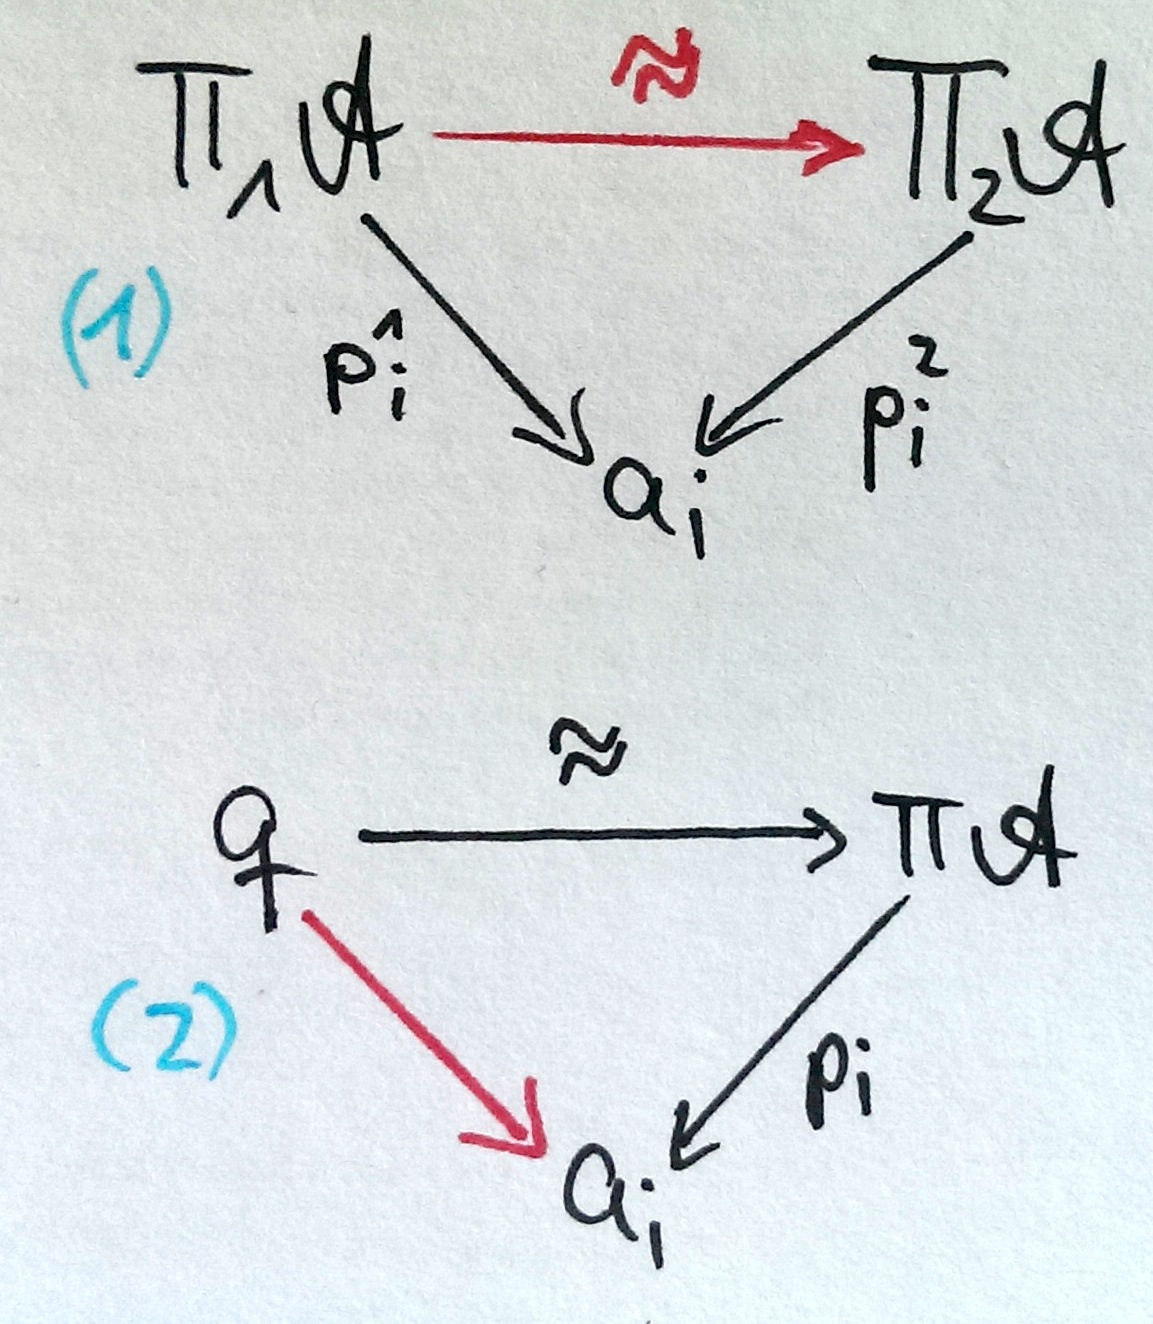
\includegraphics[width=0.29\textwidth]{Abbildungen/122}} \qquad\qquad\qquad
\subfigure[Co-Produkt\label{fig:138}]{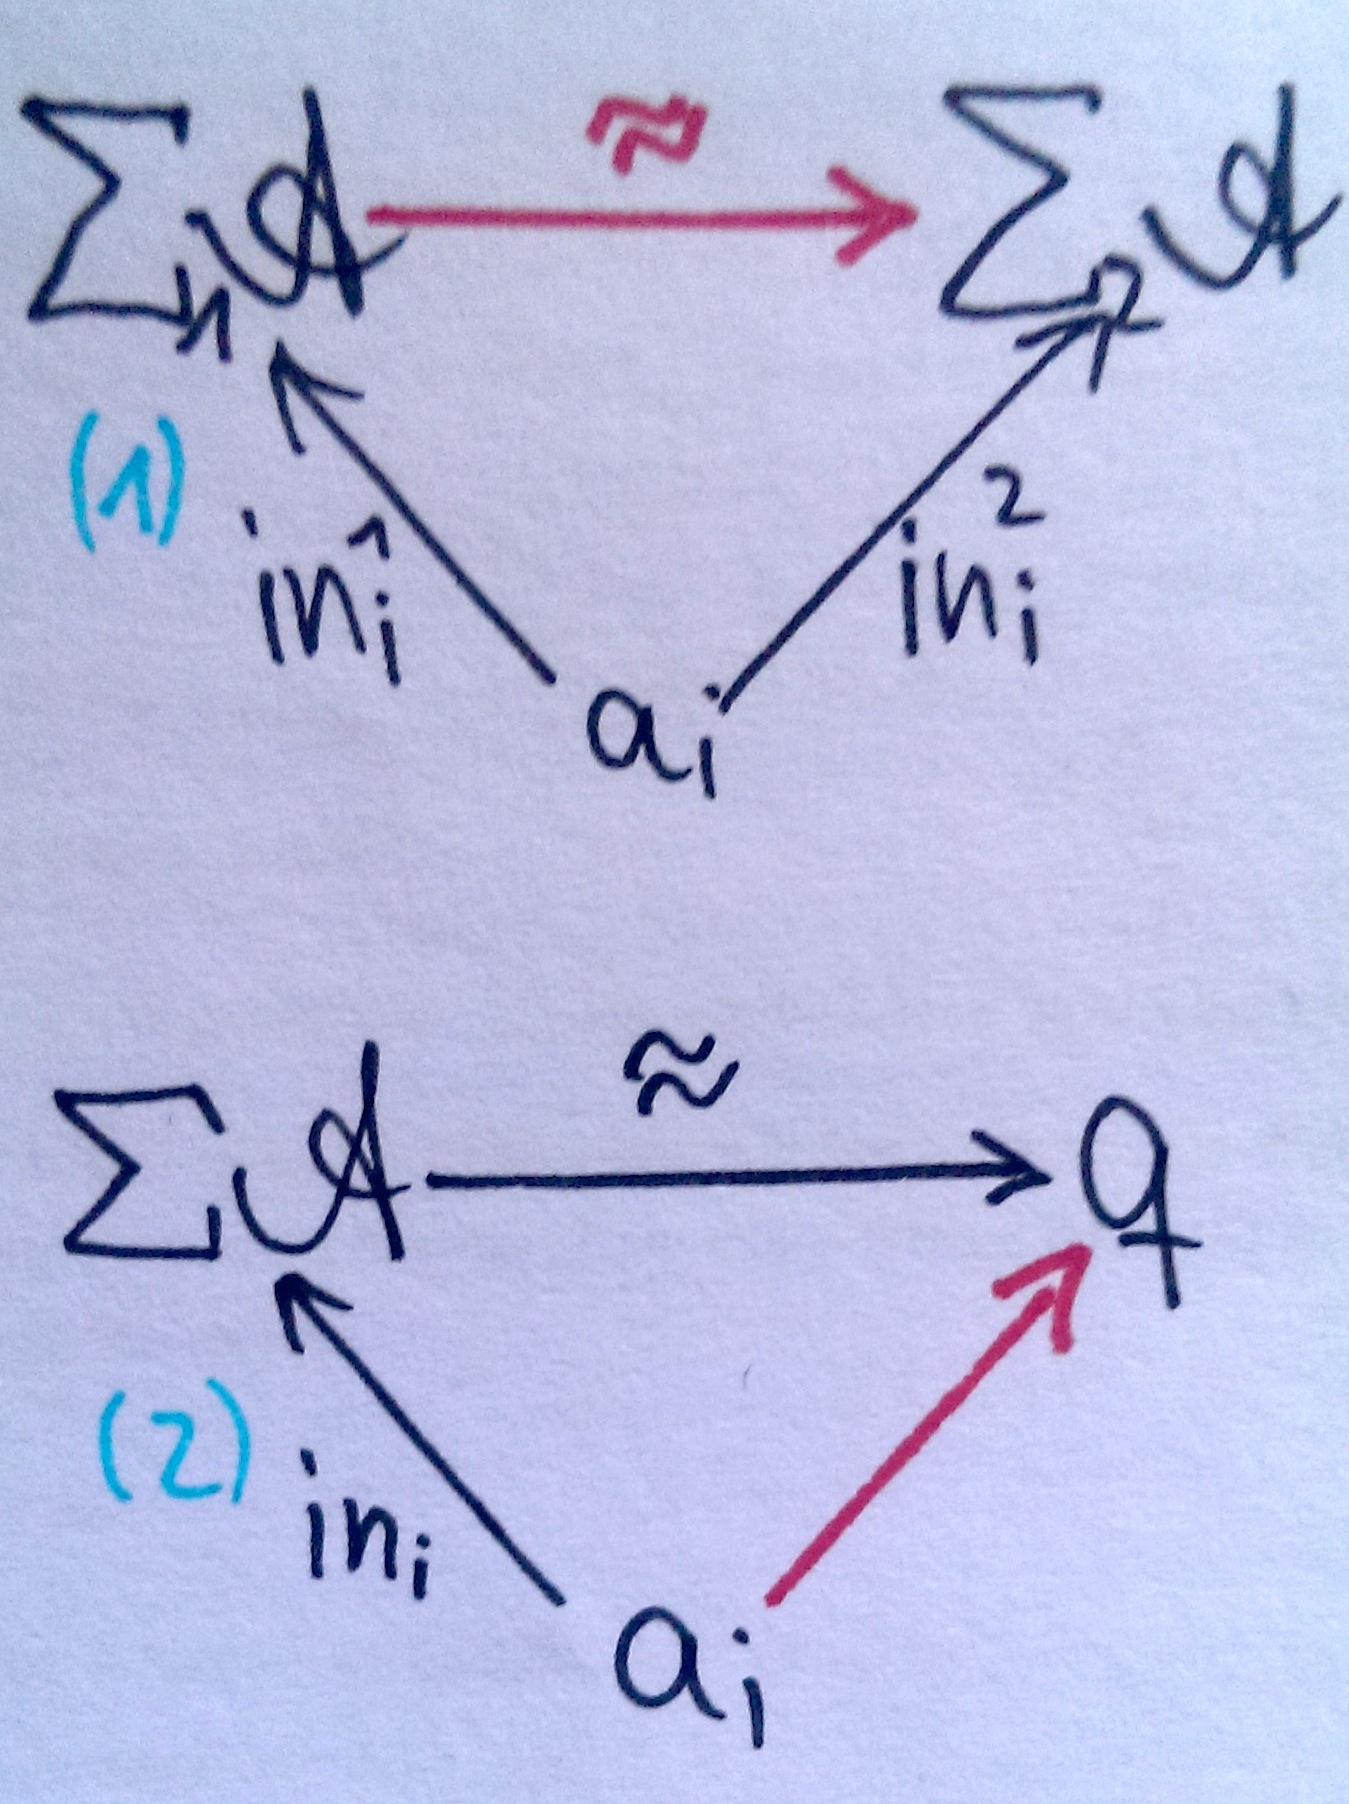
\includegraphics[width=0.24\textwidth]{Abbildungen/138}}
\caption{Abstrakte}
\end{figure}

\newpage 

\begin{multicols}{2}
\columnseprule1pt

\textbf{\underline{Produkte}} 

\textbf{\prop 123 Assoziativität und Kommutativität} \\
$\mathcal{A} = (a_i)_{i \in I}$ $\mathcal{J}$ ist Partition auf $I \Rightarrow$ $\Pi \mathcal{A} \approx \Pi(\Pi(a_i)_{i \in S})_{s \in \mathcal{J}}$ wenn alle teilnehmenden Produkte exististeren.


\textbf{\defi 125 Finales Objekt} \\
Ein Objekt $\mathcal{T}$ ist final in Kategorie $\mathcal{C}$, wenn es einen eindeutigen Morphismus von jedem anderen $\mathcal{C}$-Objekt in $\mathcal{T}$ gibt.

\textbf{\coro 126 Leeres Produkt} \\
Das finale Objekt einer Kategorie deckt sich mit dem leeren Produkt, d.h. $\mathcal{T} = \Pi \emptyset$

\textbf{\prop 127 Neutrales Element für Produktoperator} \\
Für alle Objekte $a: a \times \mathcal{T} \approx a$

\textbf{\defi 128 Produktmorphismus} \\
Geg. Fam. von Morphismen $\left(m_{i}:d_{i}\rightarrow c_{i}\right)_{i\in I}$ einer Kategorie $\mathcal{C}$ mit den Produkten \\ $D=\Pi(d_{i})_{i\in I}$
und $C=\Pi(c_{i})_{i\in I}$. \\ Der Produktmorphismus $\Pi(m_{i})_{i\in I}:D\rightarrow C$
ist der eindeutige Morphismus für die Familie von Morphismen
$\left(m_{i}\circ p_{i}:D\rightarrow c_{i}\right)_{i\in I}$,
d.h. $\Pi(m_{i})_{i\in I}=\left\langle m_{i}\circ p_{i}\right\rangle _{i\in I}$

\columnbreak

\textbf{\underline{Co-Produkte}} 

\textbf{\prop 139 Assoziativität und Kommutativität} \\
$\mathcal{A} = (a_i)_{i \in I}$ $\mathcal{J}$ ist Partition auf $I \Rightarrow$ \\ $\sum \mathcal{A} \approx \sum(\sum(a_i)_{i \in S})_{s \in \mathcal{J}}$ wenn alle teilnehmenden Co-Produkte exististeren.


\textbf{\defi 141 Initiales Objekt} \\
Ein Objekt $\mathcal{I}$ ist initial in Kategorie $\mathcal{C}$, wenn es einen eindeutigen Morphismus in jedes andere $\mathcal{C}$-Objekt von $\mathcal{I}$ gibt.

\textbf{\coro 142 Leeres Co-Produkt} \\
Das initiale Objekt einer Kategorie deckt sich mit leerem Co-Produkt, d.h. $\mathcal{I} = \sum \emptyset$

\textbf{\prop 143 Neutrales Element für Co-Produktoperator} \\
Für alle Objekte $a: a + \mathcal{I} \approx a$

\textbf{\defi 144 Co-Produkt Morphism.} \\
Geg. Fam. von Morphismen $\left(m_{i}:d_{i}\rightarrow c_{i}\right)_{i\in I}$ einer Kategorie $\mathcal{C}$ mit den Co-Produkten \\ $D=\sum(d_{i})_{i\in I}$
und $C=\sum(c_{i})_{i\in I}$. \\ Der Co-Produktmorph. $\sum(m_{i})_{i\in I}:D\rightarrow C$
ist der eindeutige Morphismus für die Familie von Morphismen
$\left(in_{i}\circ m_{i}:d_i \rightarrow C\right)_{i\in I}$,
d.h. $\sum(m_{i})_{i\in I}=\left \{in_{i}\circ m_{i}\right\} _{i\in I}$ 




\end{multicols}

\begin{figure}[h]
\centering
\subfigure[Produkt\label{fig:128}]{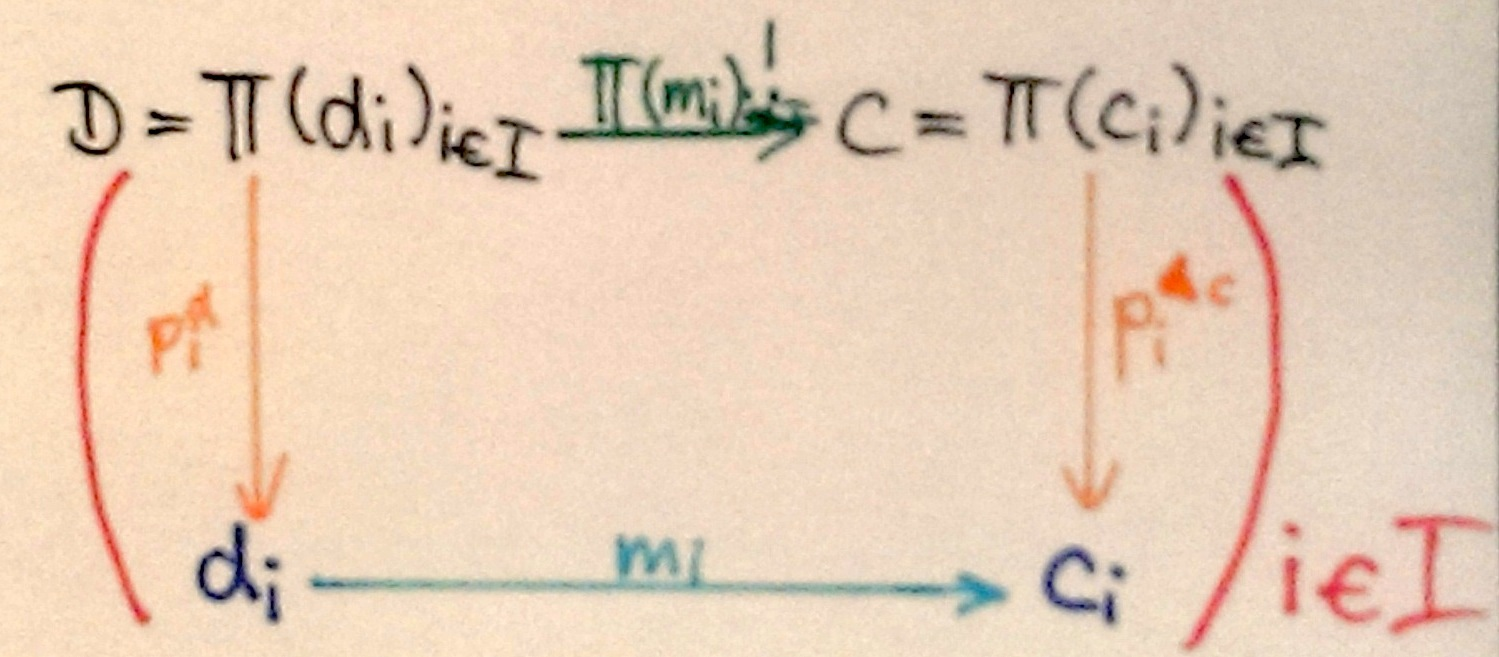
\includegraphics[width=0.41\textwidth]{Abbildungen/128}} \qquad\qquad\qquad
\subfigure[Co-Produkt\label{fig:144}]{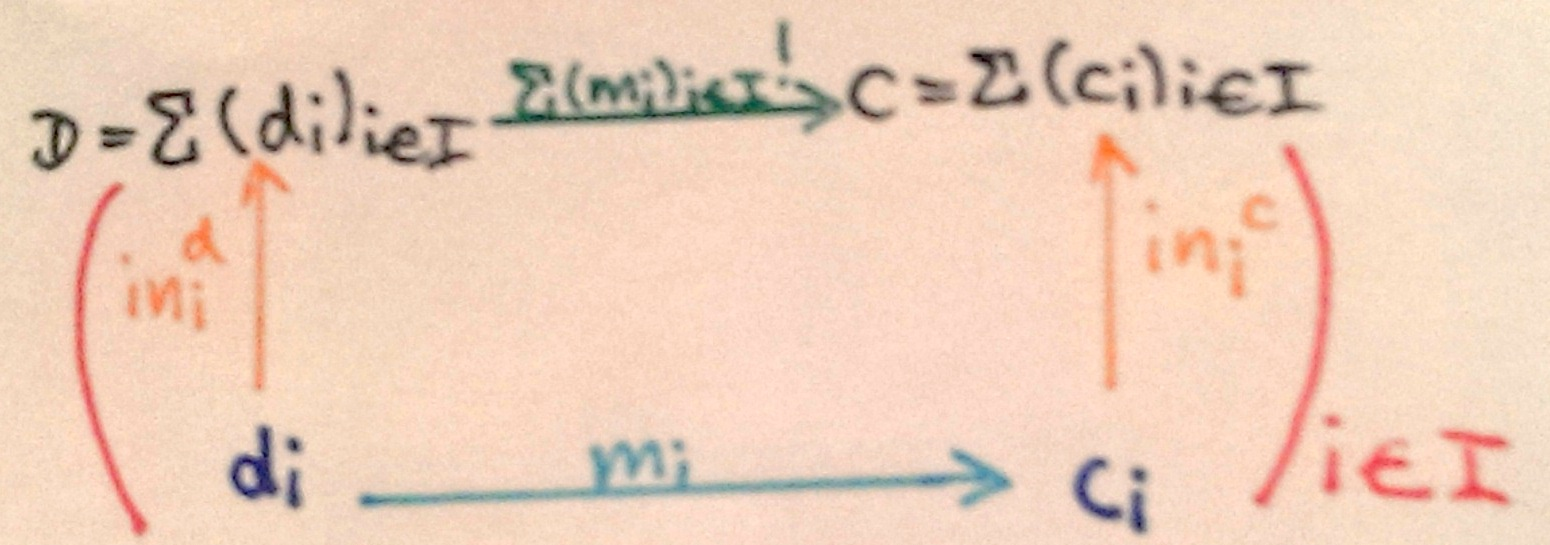
\includegraphics[width=0.41\textwidth]{Abbildungen/144}}
\caption{- Morphismus}
\end{figure}

\newpage 

\begin{multicols}{2}
\columnseprule1pt

\textbf{\underline{Produkte}} 

\textbf{\prop 129 Produkt monischer Morphismen} \\
$(m_i: d_i \rightarrow c_i)_{i \in I}$ mono $\Rightarrow \Pi(m_i)_{i\in I}: \Pi(d_i)_{i \in I} \rightarrow \Pi(c_i)_{i \in I}$ ist auch monisch.

\textbf{\prop 130 Produkt extremaler Morphismen} \\
In einer Kategorie $C$ mit Faktorisierungssystem in Epis und extremale Monos ist Produkt der extremalen Monos wieder extremal mono.

\textbf{\defi 131 Kartesisches Produkt} \\
Objekte $(a_i)_{i \in I}$ in Set. Das Produkt $\left(\Pi(a_{i})_{i\in I},\left(p_{i}:\Pi(a_{i})_{i\in I}\rightarrow a_{i}\right)_{i\in I}\right)$ ist definiert durch \\
(1) $\Pi(a_{i})_{i\in I}=\{c:I\rightarrow\bigcup_{i\in I}a_{i}\,::$\\$ \,\forall i\in I:\, c(i)\in a_{i}\}$ \\
(2) $\forall \, i\in I$ and $c\in\Pi(a_{i})_{i\in I}$: $p_{i}(c)=c(i)$

\textbf{\prop 132 Kartesisches Produkt} \\
Das Kartesische Produkt ist das Produkt in der Kategorie Set.


\textbf{\coro 133 Finales Objekt in Set} \\
Das finale Objekt in Set ist $\{*\}$.

\textbf{\defi 134 Generelle Produkte in \syssig} \\
Sei $\mathcal{A}=\left(A_{i}\right)_{i\in I}$ eine Familie algebraischer
Systeme, dann ist das Produkt $\Pi\mathcal{A}=\left(\Pi\mathcal{A},\left(p_{i}:\Pi\mathcal{A}\rightarrow A_{i}\right)_{i\in I}\right)$
definiert durch \\
(1) Produkt über alle Trägermengen \\
(2) Operationen auf Produkten ausführen die für Faktoren ausgelegt sind.\\
(3) \syssig Projektionen $p_{i,s}$ stimmen überein mit $p^{Set}_{i,s}$ 


\columnbreak

\textbf{\underline{Co-Produkte}} 

\textbf{\prop 145 Co-Produkt epischer Morphismen} \\
$(m_i: d_i \rightarrow c_i)_{i \in I}$ epi $\Rightarrow \sum(m_i)_{i\in I}: \sum(d_i)_{i \in I} \rightarrow \sum(c_i)_{i \in I}$ ist auch episch.

\textbf{\prop 146 Co-Produkt extremaler Epis} \\
In einer Kategorie $C$ mit Faktorisierungssystem in extremal Epis und Monos ist Co-Produkt der extremalen Epis wieder extremal epi.

\textbf{\defi 147 Co-Produkt in Set} \\
Objekte $(a_i)_{i \in I}$ in Set. Das Co-Produkt $\left(\sum(a_{i})_{i\in I},\left(in_{i}:a_{i} \rightarrow \sum (a_{i})_{i\in I}\right)_{i\in I}\right)$ ist definiert durch \\
(1) $\sum(a_{i})_{i\in I}=\biguplus_{i \in I} a_i$\\
(2) $\forall \, i\in I$ und $x\in a_{i} $: \\ $in_i: a_i \rightarrow \sum(a_i)_{i \in I} :: = in_i(x) = (x,i)$

\textbf{\prop 148 Co-Produkt in Set} \\
Das Co-Produkt ist das Co-Produkt in der Kategorie Set.


\textbf{\coro 149 Initiales Objekt in Set} \\
Das initiale Objekt in Set ist $\emptyset$.
\\
\\
\\
\\
\\
\\
\\
\\
\textbf{\coro 150 Initiales Objekt in \syssig} \\
Das leere algebraische System $\mathcal{I}$ ist das initiale Objekt in \syssig



\end{multicols}



\begin{multicols}{2}
\columnseprule1pt

\textbf{\underline{Produkte}} 

\textbf{\prop 135 Generelle Produkte in \syssig} \\
Das algebraische System $\Pi \mathcal{A}$ mit \\ $(p_i: \Pi \mathcal{A} \rightarrow A_i)_{i \in I}$ (aus Def 134) ist Produkt der Familie von Systemen $\mathcal{A} = (A_i)_{i \in I}$


\textbf{\coro 136 Finales Objekt in \syssig} \\
Das finale Objekt $T$ in \syssig ist das folgende algebraische System \\
(1) $(T_s = \{*\})_{s \in S}$ \\
(2) $\forall \, f \in O_{w,v} \forall \, x \in T^w: f^T(x)=*$

\columnbreak

\textbf{\underline{Co-Produkte}} 

\textbf{\prop 151 Binäres Co-Produkt in \syssig} \\
Das variante System $A + B$ ist das Co-Produkt der zwei Systeme $A$ und $B$.

\end{multicols}

% !TEX root = Zusammenfassung.tex
\chapter{Spezifikation}

\section{Abstraktion: Episch reflektive Subkategorien}

\paragraph{\defi 152: Subkategorie}
Kategorie $\mathcal{D}$ ist Subkategorie von $\mathcal{C}$ ($\mathcal{D} \subseteq \mathcal{C}$), wenn
\begin{enumerate}
\item $O^\mathcal{D} \subseteq O^\mathcal{C}$ (Objekte in Teilmengenbeziehung)
\item $\forall \, a,b \in O^\mathcal{D}:  M^\mathcal{D}_{a,b} \subseteq M^\mathcal{C}_{a,b} $
\item $\forall \, a \in O^\mathcal{D}: id^\mathcal{D}_a = id^\mathcal{C}_a$
\item $\forall \, a,b,c, \in O^\mathcal{D} \wedge m \in M^\mathcal{D}_{a,b}, n \in M^\mathcal{D}_{b,c}: n \circ^{\mathcal{D}}_{a,b,c} m  = n \circ^{\mathcal{C}}_{a,b,c} m  $
\end{enumerate}

\begin{itemize}
\item $\mathcal{D}$ ist voll, wenn
\begin{enumerate}
\item $\mathcal{D} \subseteq \mathcal{C}$ und
\item $\forall \, a,b \in O^\mathcal{D}:  M^\mathcal{D}_{a,b} = M^\mathcal{C}_{a,b} $
\end{enumerate}
\item $\mathcal{D}$ ist isomorph geschlossen, wenn $\approx: a \rightarrow b \in M^\mathcal{C}_{a,b} \text{ mit } a \in O^\mathcal{D} \implies b \in O^\mathcal{D}$
\item Wenn $\mathcal{D}$ voll und isomorph-geschlossen ist: $\mathcal{D} \subseteq^{\approx} \mathcal{C}$
\end{itemize}

Notiz: Nur isomorph-geschlossene Kategorien sind abstrakt (bis auf Isomorphie)!

\paragraph{\defi 153: Episch reflektive Subkategorie}
$\mathcal{D}$ ist reflektive Subkategorie von $\mathcal{C}$, wenn
\begin{enumerate}
\item $\mathcal{D} \subseteq \mathcal{C}$
\item $\forall \, c \in O^\mathcal{C}: $  gibt es 
\begin{itemize}
\item ein $c_\mathcal{D} $ ($\mathcal{D}$- Reflektion von $c$) und 
\item ein Morphismus $\eta_c: c \rightarrow c_\mathcal{D} $ (Reflektor von $c$) 
\end{itemize}
\end{enumerate}

mit der folgenden Eigenschaft: $\forall \,  m: c \rightarrow z$, so dass $z \in \mathcal{D}$, dann gibt es einen eindeutigen Morphismus $m^* : c_\mathcal{D} \rightarrow z$ mit $m^* \circ \eta = m$ \\
$\mathcal{D} $ ist episch reflektiv, wenn zusätzlich alle Reflektoren epis sind. 

\begin{figure}[h]
\noindent \centering{}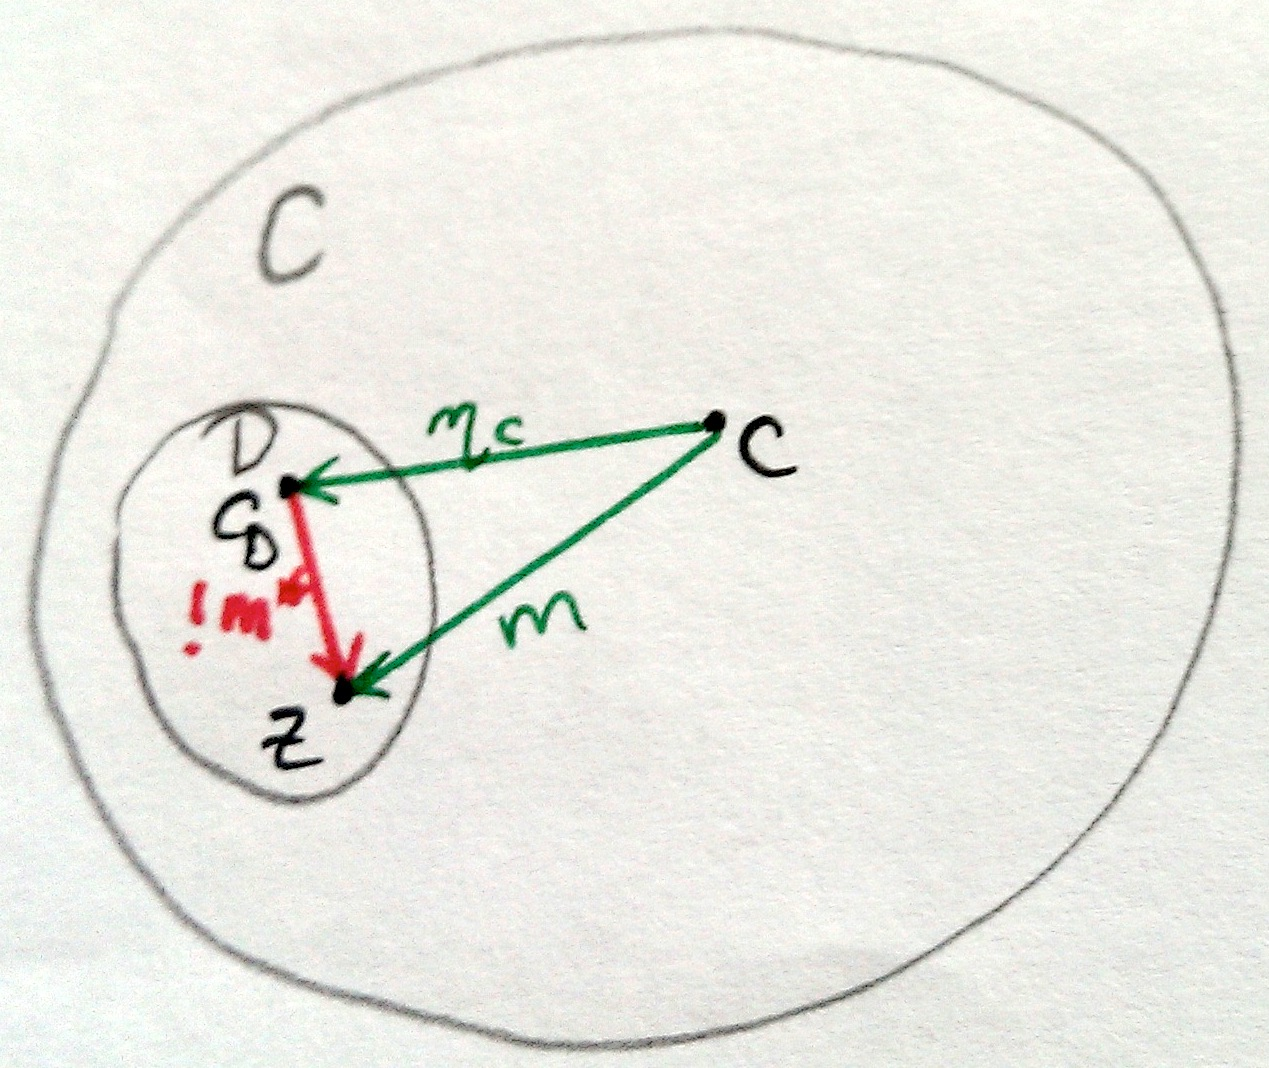
\includegraphics[scale=0.1]{Abbildungen/153}\caption{Episch reflektive Subkategorie}
\end{figure}

\paragraph{\prop 154: Reflektionen sind abstrakt}
Sei $\mathcal{D} $ reflektive Subkategorie von $\mathcal{C} $

\begin{enumerate}
\item $\eta_1: c \rightarrow c_\mathcal{D}^1 $ und $\eta_2: c \rightarrow c_\mathcal{D}^2 $ zwei Relfektionen von $\mathcal{C} \implies \approx: \mathcal{C}_\mathcal{D}^1 \rightarrow \mathcal{C}_\mathcal{D}^2 $ mit $\eta: c \rightarrow \mathcal{C}_\mathcal{D}^2$
\item  $\eta: c \rightarrow \mathcal{C}_\mathcal{D}^1$ Reflektor für $c$ und $\approx: c_\mathcal{D}^1 \rightarrow c_\mathcal{D}^2$ ist Iso $\implies \eta' \, = \, \approx \circ \eta : c \rightarrow c_\mathcal{D}^2$ ist auch Reflektor für $c$
\end{enumerate}

\begin{figure}[h]
\noindent \centering{}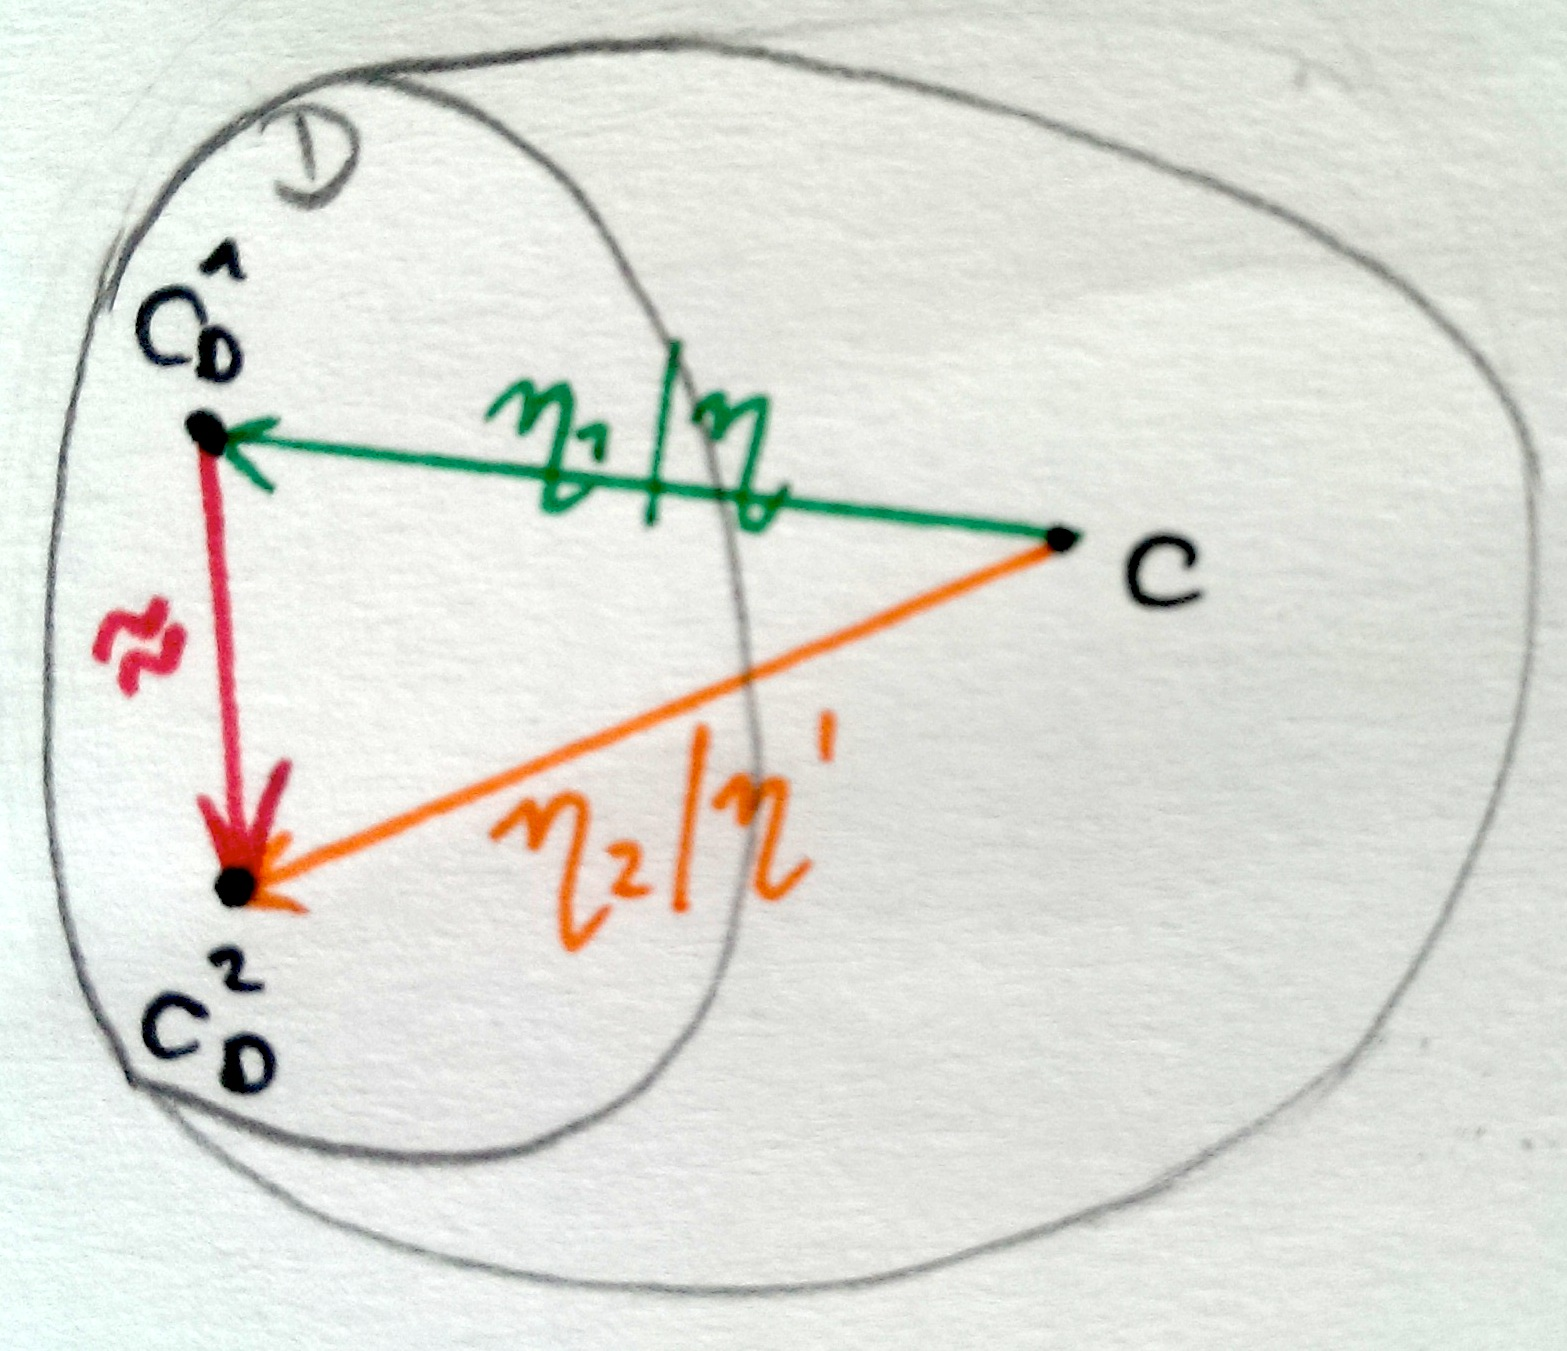
\includegraphics[scale=0.1]{Abbildungen/154}\caption{Reflektionen sind abstrakt}
\end{figure}

\paragraph{\prop 155: Isomorphe Reflektoren}
 
\begin{enumerate}
\item  $\mathcal{D} $ reflektive Subkategorie von $\mathcal{C} $ und $d \in \mathcal{D} \implies \eta_d : d \rightarrow d_\mathcal{D}$ ist iso.
\item  $\mathcal{D} $ ist reflektive und isomorph-geschlossene Subkategorie von $\mathcal{C}$ \\ $ \implies \forall \, c \in \mathcal{C}: c \in \mathcal{D} \Leftrightarrow $ der Reflektor für $c$ ist iso.  
\end{enumerate}

\paragraph{\prop 156: Epische Reflektionen und Produkte}

 $\mathcal{D}$ episch-reflektiv und isomorph-geschlossene Subkategorie von $\mathcal{C}$ und \\ $\Pi \mathcal{A}$ ist Produkt in $\mathcal{C}$ einer Familie $\mathcal{A} = (a_i)_{i \in I} $ von $\mathcal{D}$-Objekten, d.h. $(a_i \in \mathcal{D})_{i \in I}$ \\$ \implies \Pi \mathcal{A} \in \mathcal{D}$
 
 \paragraph{\prop 157: Epische Reflektionen und extremale Monos}
 $\mathcal{D}$ episch-reflektiv und isomorph-geschlossene Subkategorie von $\mathcal{C}$ mit $(\mathcal{E}, \mathcal{M}^x) \implies c \in \mathcal{D}$ wenn $m: c \rightarrowtail d$ ist extremal Mono und $d \in \mathcal{D}$. \\
 D.h. in TCs Worten: \\
 Wenn wir $\mathcal{D}$ aus Def haben und  $(\mathcal{E}, \mathcal{M}^x)$ dann folgt daraus, jedes $d$, was über einen extremalen Mono erreicht wird, hat ein 'Urbild' in $\mathcal{D}$.
 
 
\paragraph{\prop 158: Co-Well-Powered Categories}
Kategorie $\mathcal{C}$ its Co-well-powered, wenn $\forall \, a \in \mathcal{C}$ die 'Collection' abstrakter Quotienten (Def 77) von a eine Menge bildet. \\
\emph{'Colletion abstrakter Quotienten von a' = Paarweise nicht isomorphe Epis mit Domain a.}
 
 
\paragraph{Theorem 159: Charakterisierung episch reflektiver Subkategorien} 
Gegeben: $\mathcal{C}$ co-well-powered Kategorie mit ($\mathcal{E},\mathcal{M}^x$). Isomorph geschlossene Subkategorie $\mathcal{D}$ von $\mathcal{C}$i ist episch reflektiv $\Leftrightarrow \, \mathcal{D} $ geschlossen unter Produkten und extremalen Subobjekten ist. 
 
 
\paragraph{\defi 160 Reflektion von Morphismen}  
Gegeben $\mathcal{D}$ reflektive Subkategorie von $\mathcal{C}$ und $c \mapsto (\eta_c : c \rightarrow c_\mathcal{D})$ eine festgelegte Auswahl von Reflektoren $\eta_c$ für jedes Objekt $c \in \mathcal{C}$.
Dann definieren wir das folgende Mapping von Morphismen $m: c \rightarrow c' \in \mathcal{C}$ zu Morphismen in $\mathcal{D}: m : c \rightarrow c' \mapsto m^\mathcal{D}: c_\mathcal{D} \rightarrow c_\mathcal{D}' \, = \, (\eta_{c'} \circ m)^* : c_\mathcal{D} \rightarrow c_\mathcal{D}'$.  \\
\emph{In CTs Worten: Morphismen werden von $\mathcal{C}$ nach $\mathcal{D}$ reflektiert.}

\begin{figure}[h]
\noindent \centering{}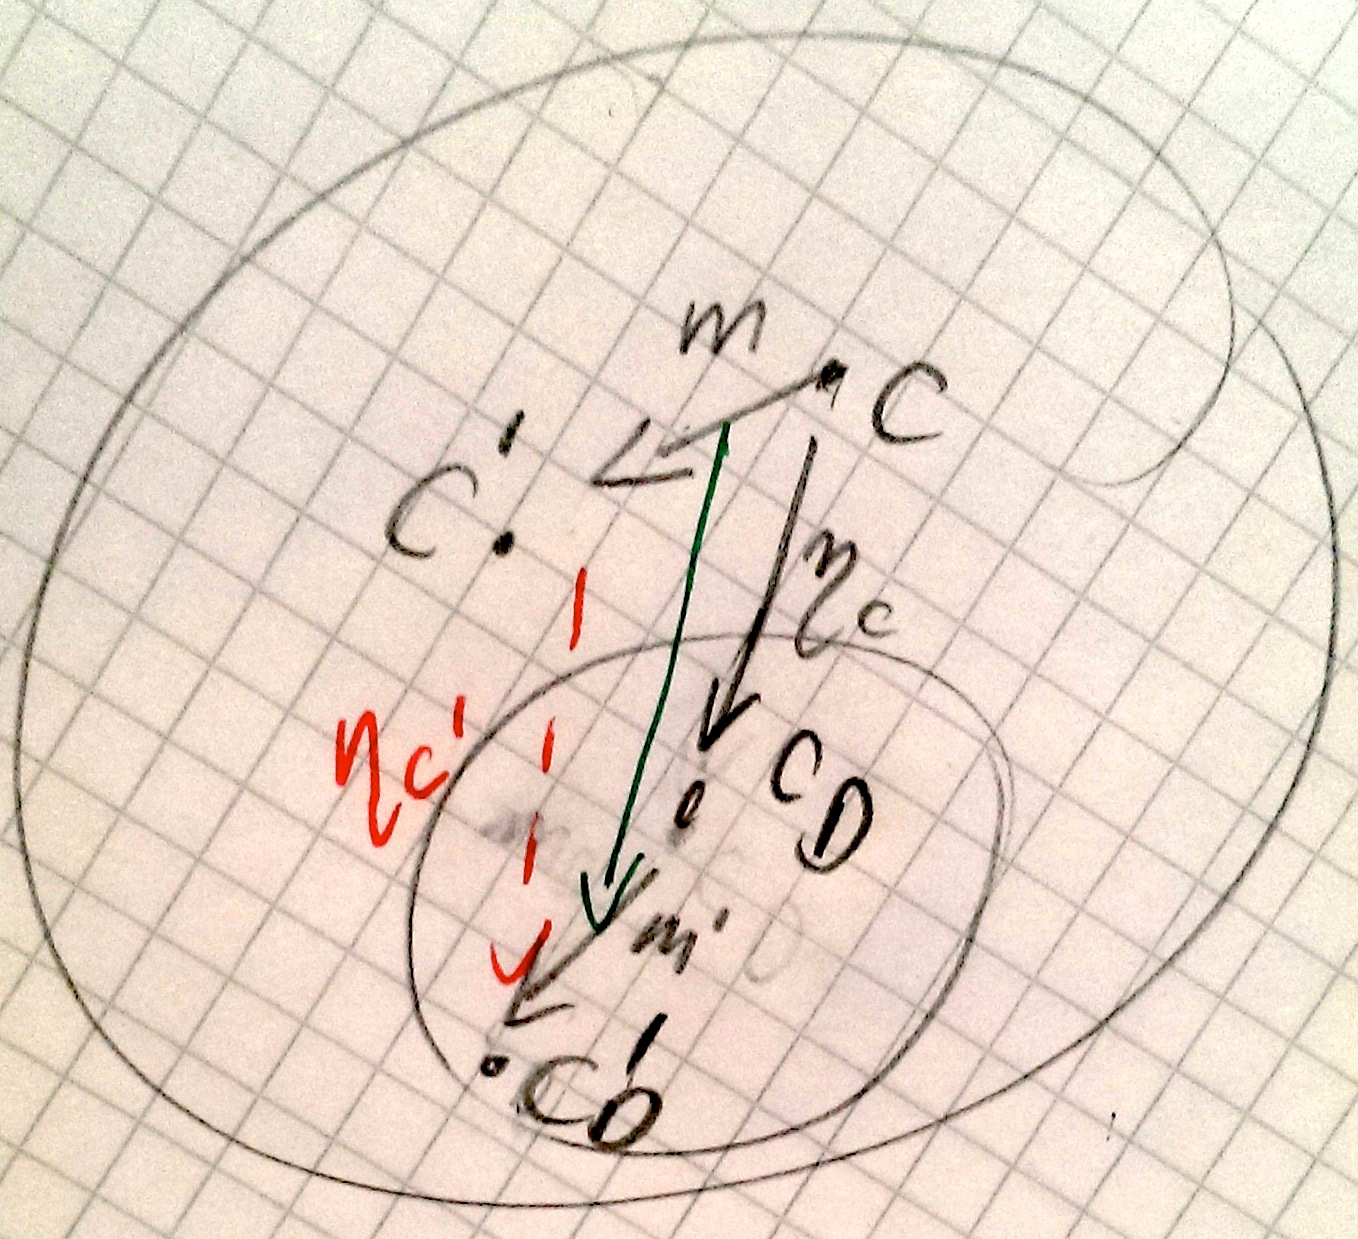
\includegraphics[scale=0.09]{Abbildungen/160}\caption{Reflektion von Monomorphismen}
\end{figure}

\paragraph{\prop 161 Eigenschaften von Morphismusreflektionen}  
$\mathcal{D}$ reflektive Subkategorie von $\mathcal{C}$ und $m \mapsto m^\mathcal{D} \Rightarrow$

\begin{enumerate}
\item $id_c^D = id_{c_\mathcal{D}}$ $\forall c \in C$
\item $(m \circ_\mathcal{C} n)^\mathcal{D} = m^\mathcal{D} \circ_\mathcal{D} n^\mathcal{D}$  wenn $m,n$ komponierbar in $C$.
\end{enumerate}
\emph{CT Notiz zu 2.: Erst verkullern und dann Übertragen ist gleich zu erst einzeln Übertragen und dann verkullern.}


\section{Syntaktifizierung}

\subsection{Terme und Termsysteme}

\paragraph{\defi 162 Variablen-Mengen und Variablen-Systeme}  
Eine Variablenmenge $X$ ist eine S-Indizierte Familie von Mengen von Variablen, d.h. $X = (X_s)_{s \in S*}$ \\
Eine Variablenmenge ist ein algebraisches System in dem alle Funktionen komplett undefiniert sind.

\paragraph{\defi 163 Terme und totale Termsysteme}
Die 'Collection' von Termen $T^{\Sigma,X}$ mit Variablen in $X$ ist die kleinste S-Indizierte Familie von Mengen $T^{\Sigma, X} = (T^{\Sigma, X}_s)_{s \in S}$ die folgende Bedingungen erfüllen:
\begin{enumerate}
\item Variablen: $x \in T^{\Sigma, X}_s $ wenn $x \in X_s$
\item Funktionen: $f_i(t) \in T^{\Sigma, X}_s $ wenn $f \in O_{w,v} $ und $t \in (T^{\Sigma, X})^w $ und $v = v_l sv_r$ und $i = |v_l| +1$

Das totale Termsystem $T^{\Sigma, X}$ mit Variablen in $X$ ist das $\Sigma$-System, welches die Familie von Termen $(T^{\Sigma, X}_s)_{s \in S}$ als Träger nehmen und alle Funktionen definieren durch:

\item Funktionen: Für $f \in O_{w,v} $ und $|v| \geq 1$ und $x \in (T^{\Sigma, X})^w: f^{T^{\Sigma, X}}(x) = (f_i(x))_{i \in 1 \dots |v|}$
\item Prädikate: Für $f \in O_{w, \epsilon}$ und $f \neq \, =: f^{T^{\Sigma, X}} = \emptyset$, d.h. $f^{T^{\Sigma, X}}$ Alle Prädikate bis auf die Gleichheit sind komplett undefiniert. 
\end{enumerate}

\emph{Notiz CT:  1. und 2. definiert die Trägermengen des totalen Termsystems \\
 Zu 3.: Ist das nicht das mit der 'Tiefe' von Termen bei Elsner? s(s(s(...))) \\
'$f \neq =$' bedeutet: f ist nur für = definiert. Sonst nichts}


\paragraph{\defi 164 Operationen auf Termen}  
Die Operationen (a) enthalten Variablen, (b) enthalten Terme und (c) die Höhe ist definiert auf der 'Collection' von Termen $T^{\Sigma, X}$ durch:

1. Fall: Variablen \\
2. Fall: Rekursiver Aufruf für Operationen mit Termen \\
3. Fall: Konstanten \\
4. Fall: Wenn Variable Kreuzprodukt \\

\begin{align*}
\textrm{\_}_{X}:\left(T^{\Sigma,X}\right)^{w}\rightarrow2^{X}\!::=\, & t_{X}=\begin{cases}
\{t\} & t\in X\\
x_{X} & t=f_{i}(x),f\in O_{w,v},1\leq i\leq|v|\\
\emptyset & t\in\left(T^{\Sigma,X}\right)^{\epsilon}\\
x_{X}^{1}\cup x_{X}^{2} & t=x^{1}\times x^{2}
\end{cases} & \textrm{\!(a)}\\
\textrm{\_}_{T}:\left(T^{\Sigma,X}\right)^{w}\rightarrow2^{T^{\Sigma,X}}\!::=\, & t_{T}=\begin{cases}
\{t\} & \! t\in X\\
\{f_{j}(x)::j\in[1,|v|]\}\cup x_{T} & \! t=f_{i}(x),f\in O_{w,v},i\in[1,|v|]\\
\emptyset & \! t\in\left(T^{\Sigma,X}\right)^{\epsilon}\\
x_{T}^{1}\cup x_{T}^{2} & \! t=x^{1}\times x^{2}
\end{cases} & \textrm{\!(b)}\\
|\textrm{\_|:}\left(T^{\Sigma,X}\right)^{w}\rightarrow\mathbb{N}_{0}\!::=\, & |t|=\begin{cases}
0 & t\in X\\
|x|+1 & t=f_{i}(x),f\in O_{w,v},1\leq i\leq|v|\\
0 & t\in\left(T^{\Sigma,X}\right)^{\epsilon}\\
\max(|x^{1}|,|x^{2}|) & t=x^{1}\times x^{2}
\end{cases} & \textrm{\!(c)}
\end{align*}

\paragraph{\defi 165 Partielle Termsysteme}  
Ein partielles Termsystem $P^{\Sigma,X}$ ist ein Subsystem von dem totalen Termsystem $T^{\Sigma,X}$, so dass 
\begin{enumerate}
\item $X \subseteq P^{\Sigma,X}$
\item $\left\lceil X\right\rceil _{P^{\Sigma,X}}^{c}$ (Wenn Argumente des Terms selber wieder Terme sind, sind diese auch in $P^{\Sigma,X}$ enthalten)
\end{enumerate}

\paragraph{\coro 166 Variablen-Einbettung und eindeutiger Homomorphismus}  
\begin{enumerate}
\item Für jedes partielle System $P^{\Sigma,X}$ die Einbettung $X\hookrightarrow P^{\Sigma,X}$ ist epi.
\item $h^1, h^2: P^{\Sigma,X} \rightarrow A$ homo eines partiellen Systems $P^{\Sigma,X}$ in ein anderes algebraisches System $A \implies h_{|X|}^1 = h_{|X|}^2 \implies h^1 = h^2$, d.h. wenn die Homos $h_1$ und $h_2$ in den Variablen übereinstimmen, sind sie gleich.  
\end{enumerate}

\paragraph{\prop 167 Struktur des partiellen Systems}
Die Menge aller partiellen Systeme $P^{\Sigma,X}$ stimmt bis auf einer Variablenmenge $X$ überein mit einem kompletten Verband bis auf die Subsystem-Relation.

\paragraph{\prop 168 Generiertes Termsystem}
Gegeben: $X$ und eine Familie von Termmengen $\mathsf{T}=\left(\mathsf{T}_{s}\subseteq T_{s}^{\Sigma,X}\right)_{s\in S}$,
$P_{\mathsf{T}}^{\Sigma,X}$ beschreibt das kleinste partielle Termsystem
das alle Terme in  $\mathsf{T}$ beinhaltet, d.h. ~$P_{\mathsf{T}}^{\Sigma,X}=\bigcap\left\{ P^{\Sigma,X}\in\mathcal{P}^{\Sigma,X}\,::\,\left(\mathsf{T}_{s}\subseteq P_{s}^{\Sigma,X}\right)_{s\in S}\right\}$\footnote{$\mathcal{P}$ ist eine Menge von partiellen Termsystemen} 


\paragraph{\prop 169 Konstruktion von generierten Termsystemen}
$\mathsf{T}=\left(\mathsf{T}_{s}\subseteq T_{s}^{\Sigma,X}\right)_{s\in S}$,
die Träger von $P_{\mathsf{T}}^{\Sigma,X}$ können wie folgt konstruiert werden
$\underset{t\in\mathsf{T}}{\bigcup}t_{T}$.


\paragraph{\prop 170 Generiertes Termsystemen}
Das generierte Termsystem hat die folgenden Eigenschaften: 
\begin{enumerate}
\item $\mathsf{T}\subseteq P_{\mathsf{T}}^{\Sigma,X}$
\item $\mathsf{T}_{1}\subseteq\mathsf{T}_{2}\implies P_{\mathsf{T}_{1}}^{\Sigma,X}\subseteq^{f}P_{\mathsf{T}_{2}}^{\Sigma,X}$.
\item $P_{\left(P_{\mathsf{T}}^{\Sigma,X}\right)}^{\Sigma,X}=P_{\mathsf{T}}^{\Sigma,X}$
\end{enumerate}

\paragraph{\prop 171 Variablenzuweisung und Erweiterungen von Variablenzuweisungen} 
\begin{enumerate}
\item Geg. $X$, $\Sigma$-System $A$: Eine Variablenzuweisung ist ein Homomorphismus $h: X \rightarrow A$
\item $P^{\Sigma,X}$ mit Variablen in $X$, mit der Variableneinbettung $x: X \hookrightarrow P^{\Sigma,X}$ und $h: X \rightarrow A$ ist eine Variablenzuweisung in $A$. \\
$\implies$ wenn er existiert, wird der eindeutige Homomorphismus, der die Variablenzuweisung zu $P^{\Sigma,X}$ erweitert,  bezeichnet mit $h^*: P^{\Sigma,X} \rightarrow A$, d.h. $h^*$ ist der einzige Homomorphismus, der $h^* \circ x = h $ erfüllt.
\end{enumerate}

\paragraph{\defi 172 Auswertung} 
Gegeben Variablenzuweisung $h: X \rightarrow A$. Partielles Termsystem $P(h) = (P(h)_s)_{s \in S} \subseteq T^{\Sigma,X}$, genannt die Auswertungsdomain von $h$, und die Auswertung $h*: P(h) \rightarrow A = (h_s^*: P(h)_s \rightarrow A_s)_{s \in S}$ selbst, sind wie folgt definiert:
$P(h)$ ist das kleinste partielle Termsystem das das folgende erfüllt: 
\begin{align*}
\textrm{(i) } & x\in P(h)_{s}\textrm{ if }x\in X_{s}\\
\textrm{(i') } & h_{s}^{*}(x)=h_{s}(x)\textrm{ for }x\in X_{s}\\
\textrm{(ii) } & f_{i}(x)\in P(h)_{s}\textrm{ if }f\in O_{w,v},v=v_{l}sv_{r},i=|v_{l}|+1,x\in\left(P(h)\right)^{w}\textrm{ and }f^{A}\textrm{ defined }\textrm{for }\left(h^{*}\right)^{w}(x)\\
\textrm{(ii') } & h_{s}^{*}(f_{i}(x))=f^{A}\left(\left(h^{*}\right)^{w}(x)\right)_{i}\textrm{ if }f\in O_{w,v},f_{i}(x)\in P(h)_{s}
\end{align*}

\paragraph{\prop 173 Auswertungshomomorphismus}
Die Auswertung $h^*: P(h) \rightarrow A$, die für die Variablenzuweisungen $h: X \rightarrow A$ (nach Def 172) definiert ist, ist ein Homo.
 
\paragraph{\coro 174 Auswertungen und Homomorphismen}
$k: A \rightarrow B$ ist Homo und $h: X \rightarrow A$ Variablenzuweisung $\Rightarrow$
\begin{enumerate}
\item $P(h) \subseteq P(k \circ h)$
\item $k  \circ h^* = (k \circ h)^* \circ \subseteq_k$, wenn der Inklusionsmorphismus von $P(h)$ in $P(k \circ h)$ bezeichnet wird durch $\subseteq_{k}: P(h) \rightarrow P(k \circ h)$
\end{enumerate}

\paragraph{\coro 175 Auswertungen und geschlossene Monomorphismen}
$k: A \rightarrow B$ geschlossener Mono und $h: X \rightarrow A$ Variablenzuweisung $\Rightarrow$
\begin{enumerate}
\item $P(h) = P(k \circ h)$
\item $k  \circ h^* = (k \circ h)^*$
\end{enumerate}

\paragraph{\coro 175 Auswertungen und Epimorphismen} 
$e: B \twoheadrightarrow C$ ist epi $\implies e^*: P(e) \rightarrow C$ ist surjektiv.


\subsection{Formeln und syntaktische Präsentation}

\paragraph{\defi 177 Atomare Formeln} 
Die Menge atomarer Formeln $F^{\Sigma,X} = (P^{\Sigma,X}_s)_{s \in S \cup \{ \epsilon\}}$ über einer gegebenen Variablenmenge $X$ ist die kleinste Menge die folgende Klauseln definiert wird:
\begin{enumerate}
\item Existenzformeln: $t \in F^{\Sigma,X}_s$, wenn $t \in T^{\Sigma,X}_s$
\item Atomare Formeln: $f(t) \in F^{\Sigma,X}_{\epsilon}$, wenn $f \in O_{w,\epsilon}$, $t \in (T^{\Sigma,X})^w$
\end{enumerate}

\paragraph{\defi 178 Operatoren auf Formeln} 
Die Operatoren \emph{beinhaltete Variablen}$(\__X)$, \emph{beinhaltete Terme}$(\__T)$, \emph{Höhe}$(|\_|)$ können auf Formeln und Familien von Formeln durch die folgenden zusätzlichen Definitionen erweitert werden:
\begin{eqnarray*}
\textrm{\_}_{X}:F_{\epsilon}^{\Sigma,X}\rightarrow2^{X} & ::= & f(x)_{X}=x_{X}\\
\textrm{\_}_{X}:2^{F^{\Sigma,X}}\rightarrow2^{X} & ::= & F_{X}=\left.\bigcup\right._{a\in F}a_{X}\\
\textrm{\_}_{T}:F_{\epsilon}^{\Sigma,X}\rightarrow2^{T^{\Sigma,X}} & ::= & f(x)_{T}=x_{T}\\
\textrm{\_}_{T}:2^{F^{\Sigma,X}}\rightarrow2^{X} & ::= & F_{T}=\left.\bigcup\right._{a\in F}a_{T}\\
|\textrm{\_|:}F_{\epsilon}^{\Sigma,X}\rightarrow\mathbb{N}_{0} & ::= & |f(x)|=|x|
\end{eqnarray*}

\paragraph{\defi 179 Syntaktische Präsentation}
Eine syntaktische Präsentation $F = (X, F \subseteq F^{\Sigma,X})$ eines algebraischen System $A$ besteht aus der Variablenmenge $X$ und der Menge von Formeln $F$ über $X$, welche gültig im präsentierten System sind.
Eine Präsentation endlich, wenn $X$ und $F$ endlich sind.
Wenn

\begin{enumerate}
\item $\mathsf{T}=F_{T}$ in die Menge von Termen die in $F$ auftreten,
\item $P_{\mathsf{T}}^{\Sigma,X}$ ist das partielle Termsystem definiert durch  $\mathsf{T}$ und
\item $P_{\mathsf{F}}^{\Sigma,X}$ ist das kleinste Supersystem von  $P_{\mathsf{T}}^{\Sigma,X}$, wo, für allel $f\in O_{w,\epsilon}$
und  $f\neq\,\,=$, $f^{P_{\mathsf{F}}^{\Sigma,X}}(x)$ definiert ist, wenn 
$f(x)\in F$ \\
$\implies$ dann wird das \emph{System} $A_{F}$, welches durch $F$  \emph{präsentiert} wird,
wird  definiert durch $\mathbf{A}_{F}=\left(P_{\mathsf{F}}^{\Sigma,X}\right)_{|\equiv_{F}}$, wobei
\item $\equiv_{F}$ ist die durch $\sim_{F}=\{(x_{1},x_{2})\,::\,\,\,\,=(x_{1},x_{2})\,\in F\}$ generierte Kongruenz,
welche die Menge der Gleichheiten, die durch $F$ spezifiert sind, ist.
\end{enumerate}

Der Epimorphismus $x^F = \, \equiv_{F}\circ\subseteq_{\mathsf{F}}\circ\, x:X\rightarrow\mathbf{A}_{F}$
definiert durch folgende Epis: %
\begin{itemize}
\item $x:X\rightarrow P_{\mathsf{T}}^{\Sigma,X}$
\item $\subseteq_{\mathsf{F}}:P_{\mathsf{T}}^{\Sigma,X}\rightarrow P_{\mathsf{F}}^{\Sigma,X}$ und 
\item $\equiv_{F}:P_{\mathsf{F}}^{\Sigma,X}\rightarrow\mathbf{A}_{F}$  
\end{itemize}
 
 \newpage 
\paragraph{\prop 180 Sub-Präsentationen}
$(X^1, F^1)$ ist Sub-Präsentation von $(X^2, F^2)$ im Sinne von $X^1 \subseteq X^2$ und $F^1 \subseteq F^2$ mit den Einbettungshomo $i: X^1 \rightarrow X^2$ \\
$\implies $ es gibt einen eindeutigen Homo $i^*: \mathbf{A}_{F^1} \rightarrow \mathbf{A}_{F^2}$ mit $i^* \circ x^{F^1} = x^{F^2} \circ i$

\begin{figure}[h]
\noindent \centering{}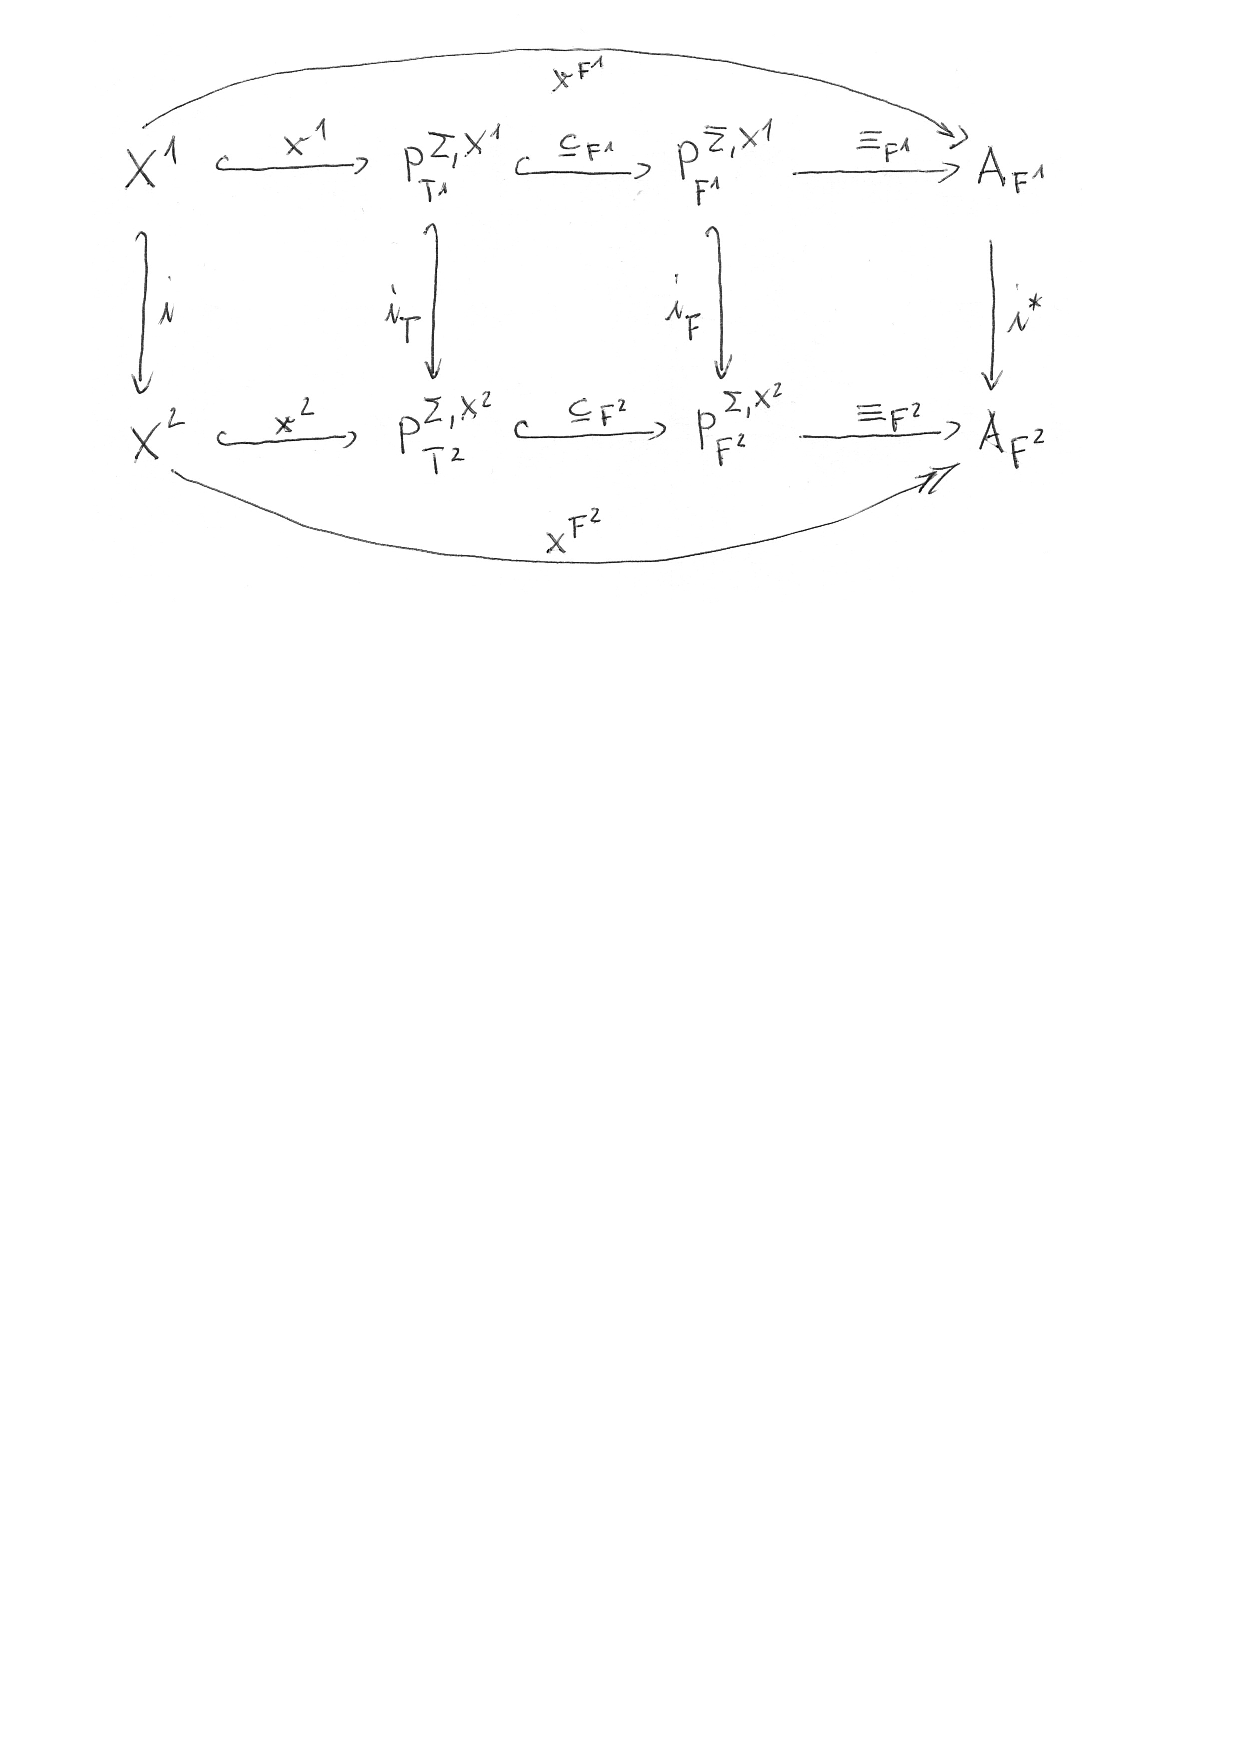
\includegraphics[scale=0.5]{Abbildungen/180}\caption{Sub-Präsentationen}
\end{figure}

\paragraph{\defi 181 Erweiterte Auswertung}
Gegeben $h: X \rightarrow A$ Variablenzuweisung. $F(h) = (X,(F(h)_s)_{s \in S \cup \{\epsilon\}}$ (Syntaktische Präsentation des geschlossenen Sub-Systems von $A$, welches generiert wurde durch $h(X)$) ist die kleinste Menge von Formeln definiert durch
\begin{enumerate}
\item $(F(h)_s = P(h)_s)_{s \in S}$ und 
\item $f(x) \in F(h)_\epsilon$, wenn $f \in O_{w, \epsilon}$, $f \in P(h)^w$, und $f^A$ ist definiert für $(h*)^w(x)$
\end{enumerate}

\paragraph{\coro 182 Erweiterte Auswertung und Homos}
$k: A \rightarrow B$ ist Homo und $h: X \rightarrow A$ Variablenzuweisung $\implies $ $F(h) \subseteq F(k \circ h)$

\paragraph{\coro 183 Syntaktische Präsentation für ein System}
$\mathbf{A}_{F(id_A)} \approx A$, wobei $id_A: (A_s)_{s \in S} \rightarrow A$ ist die identische Variablenzuweisung definiert durch $a \mapsto a$ für alle $a \in (A_s)_{s \in S*}$

\paragraph{\coro 184 Syntaktische Präsentation von Epis}
$e: B \twoheadrightarrow C$ ist epi $\implies \mathbf{A}_{F(e)} \approx C$ und $\approx \circ x^{F(e)} = e$


\section{Approximation}
\subsection{kommt nix}
\subsection{kommt nix}
\subsection{Pushout und Pullback}

\paragraph{\defi 206 Span, Co-Span}
In einer Kategorie $\mathcal{C}$: \\Span ist ein Paar $(p,q)$ von Morphismen mit der selben Domain. \\
Co-Span ist so ein paar mit der selben Co-Domain. \\ 
 \emph{Notiz: Span ist ein Diagramm von Graphen $\bullet \leftarrow \bullet \rightarrow \bullet$ und ein Co-Span \\ ist ein Diagramm von $\bullet \rightarrow  \bullet \leftarrow \bullet$ }

\begin{multicols}{2}
\columnseprule1pt

\textbf{\underline{Pushout}} 

\textbf{\defi 207 Pushout} \\
Ein Pushout eines Span $(P: a \nach b, q: a \nach c)$ ist ein Paar von Morphismen $(p^*: c \nach d, q^*: b \nach d)$, so dass $(p^*, q^*, p^* \circ q = q^* \circ p)$ ist der Co-Limit des Span. \\
\emph{Notiz: Zwei Morphismen $p^*$ und $q^*$ Charakterisieren den Co-Limes, der dritte $p^* \circ q = q^* \circ p$ kann von der Co-Cone-Eigenschaft abgeleitet werden.}

\textbf{\coro 208 Pushout Komposition} \\
\ref{fig:208} ist kommutatives Diagramm und $(1)$ ist Pushout, dann $(2)$ ist Pushout $\Leftrightarrow$ das ganze Diagramm $(1)+(2)$ ist ein Pushout.




\columnbreak

\textbf{\underline{Pullback}} 

\textbf{\defi 216 Pullback} \\
Ein Pullback eines Co-Span $(p: b \nach a, q: c \nach a)$ ist ein Paar von Morphismen $(p^*: d \nach c, q^*: d \nach b)$, so dass $p^*,q^*, q \circ p^* = p \circ q^*$ ist der Limit des Co-Span.

\textbf{Weitere Pullbacks...} \\
Weitere siehe Skript.

\end{multicols}

\begin{figure}[h]
\centering
\subfigure[Pushout\label{fig:208}]{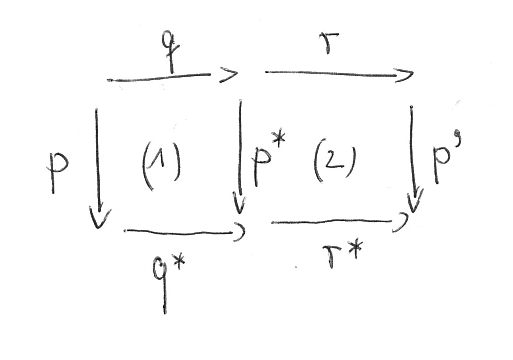
\includegraphics[width=0.21\textwidth]{Abbildungen/208}} \qquad \qquad \qquad
\subfigure[Pullback\label{fig:217}]{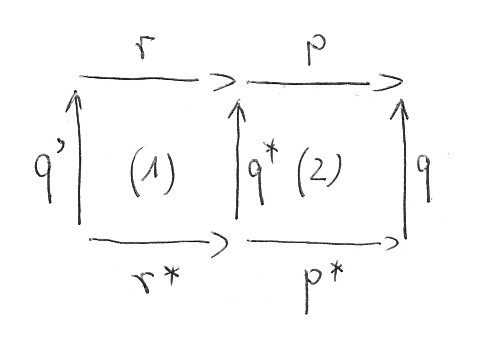
\includegraphics[width=0.20\textwidth]{Abbildungen/217}}
\caption{Definitionen}
\end{figure}


\begin{multicols}{2}
\columnseprule1pt

\textbf{\underline{Pushout}} 

\textbf{\coro 209 Pushout Dekomposition} \\
In einer Kategorie, in welcher jeder Span ein Pushout hat kann der Pushout ($p^*, (r \circ q)^*$) des Span $(p, r \circ q)$ dekomponiert werden in zwei Produkte 
\begin{enumerate}
\item $(p' q^*)$ von $(p,q)$ und 
\item $(p^*, r^*)$ von $(p', r)$, so dass \\ $(r \circ q)^* = r^* \circ q*$
\end{enumerate}

\textbf{\coro 210 Pushouts bewahren Epis} \\
$(p^*, q^*)$ ist Pushout $(p,q)$ und $p$ ist Epi.\\
$\implies p^*$ ist epi.


\columnbreak

\textbf{\underline{Pullback}} 

\textbf{Weitere Pullbacks...} \\
Weitere siehe Skript.

\end{multicols}

\begin{figure}[h]
\centering
\subfigure[Pushout\label{fig:209}]{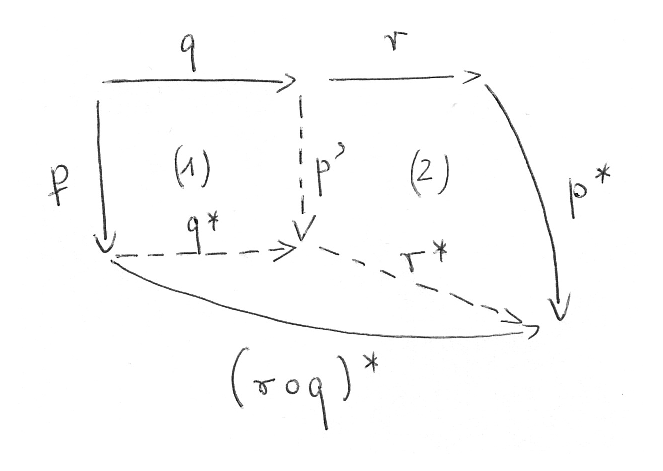
\includegraphics[width=0.22\textwidth]{Abbildungen/209}} \qquad \qquad \qquad
\subfigure[Pullback\label{fig:todo}]{
\includegraphics[width=0.22\textwidth]{Abbildungen/todo}}
\caption{Dekomposition}
\end{figure}

\begin{figure}[h]
\centering
\subfigure[Pushouts und Epis\label{fig:210}]{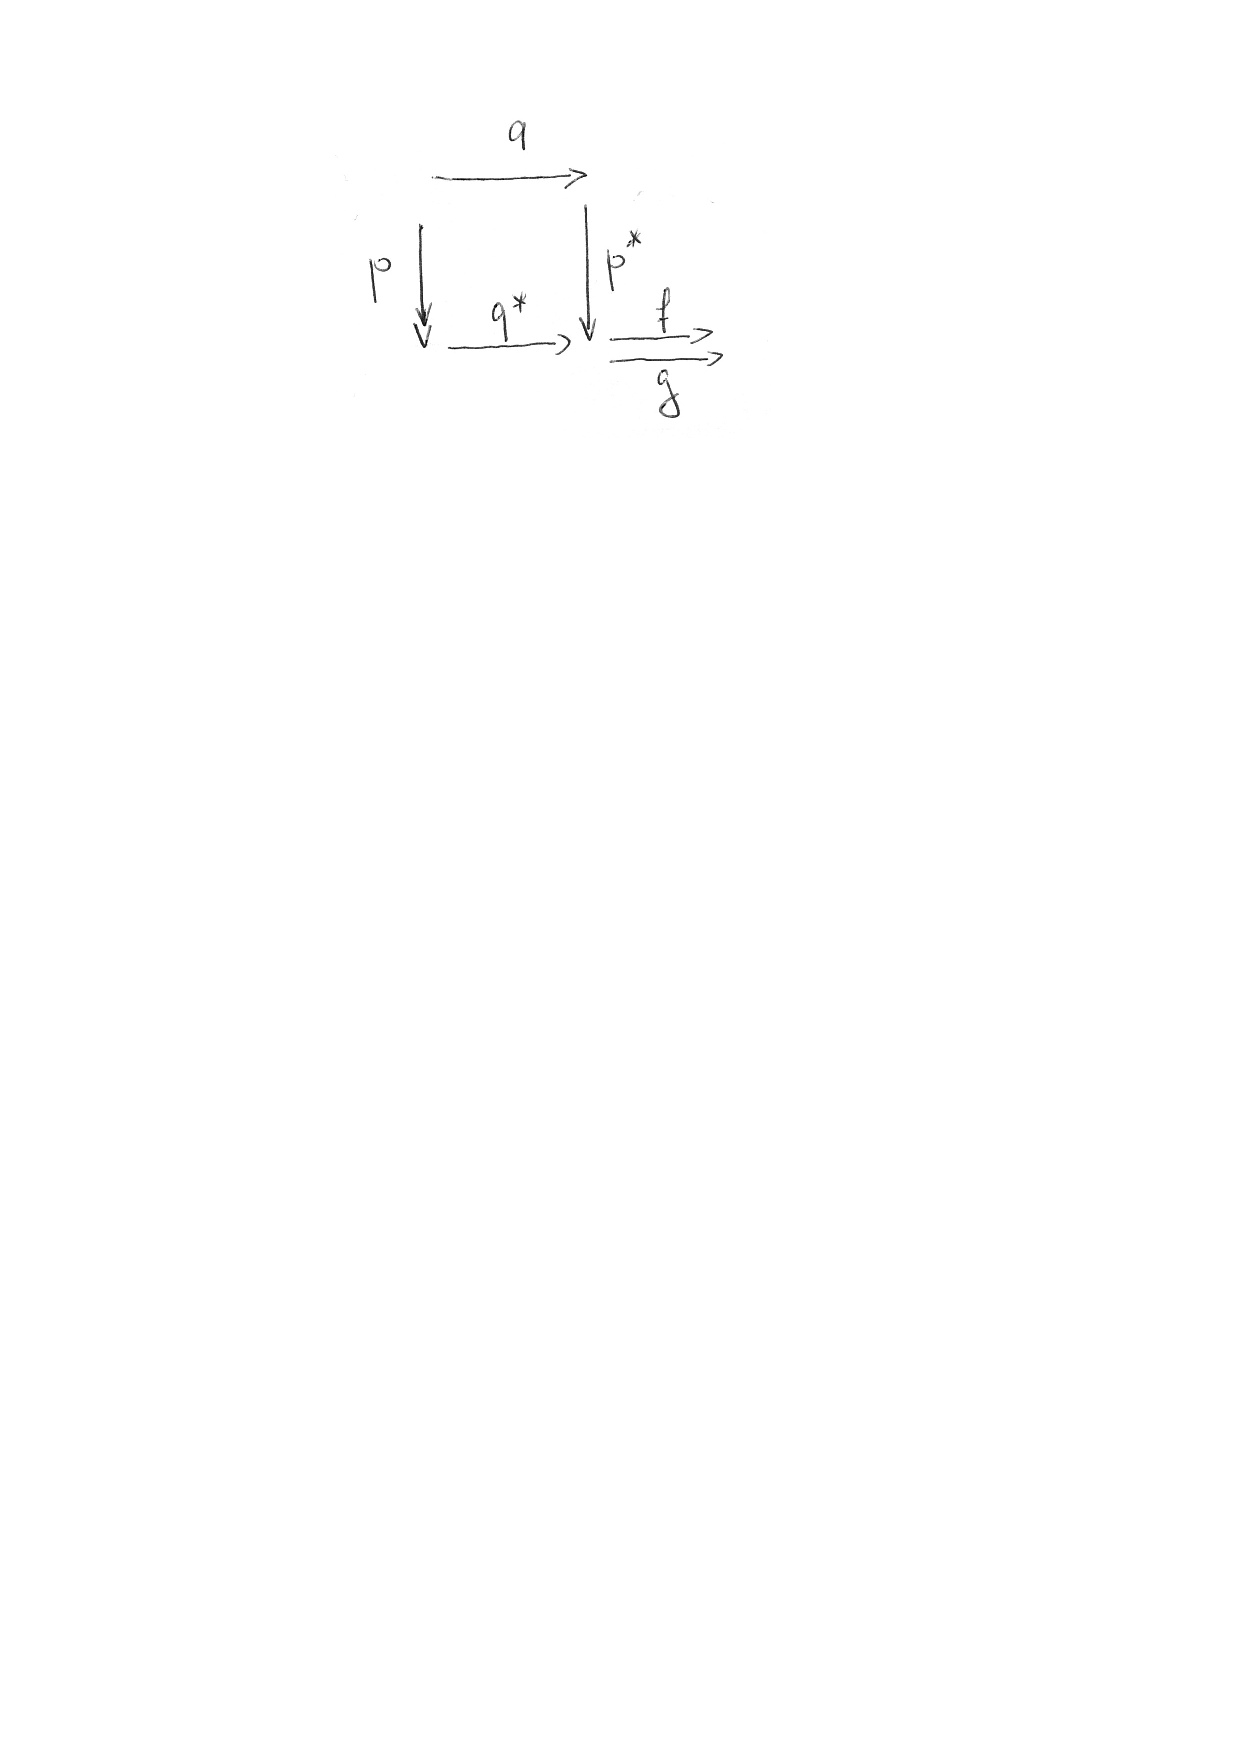
\includegraphics[width=0.22\textwidth]{Abbildungen/210}} \qquad \qquad \qquad
\subfigure[Pullback\label{fig:todo}]{
\includegraphics[width=0.22\textwidth]{Abbildungen/todo}}
\caption{Pushouts und Pullbacks}
\end{figure}

\newpage 

\begin{multicols}{2}
\columnseprule1pt

\textbf{\underline{Pushout}} 

\textbf{\prop 211 Pushouts bewahren extremale Epis} \\
Die zugrundeliegende Kategorie $(\mathcal{C})$ hat ein $(\mathcal{E}^x, \mathcal{M})$, $(p^*, q^*)$ ist Pushout von $(p,q)$ und $p$ ist extremal Epi $\implies$ $p^*$ ist extremal Epi.

\textbf{\prop 212 Pushouts bewahren Sektionen} \\
$(p^*, q^*)$ ist Pushout von $(p,q)$ und $p$ ist Sektion $\implies $ $p^*$ ist Sektion.

\textbf{\coro 213 Abgeleitete Pushouts} \\
$(p^*, q^*)$ ist Pushout von $(p,q)$, wobei $p$ Sektion $\implies$ $\left ( q, (p^*)^{-1} \right )$ ist Pushout von $(q^*, p^{-1})$, wenn wir $(p^*)^{-1}$ als das eindeutige $u$ in Prop 212 wählen.

\columnbreak

\textbf{\underline{Pullback}} 

\textbf{Weitere Pullbacks...} \\
Weitere siehe Skript.

\end{multicols}


\begin{figure}[h]
\centering
\subfigure[Pushouts und extremal Epi\label{fig:211}]{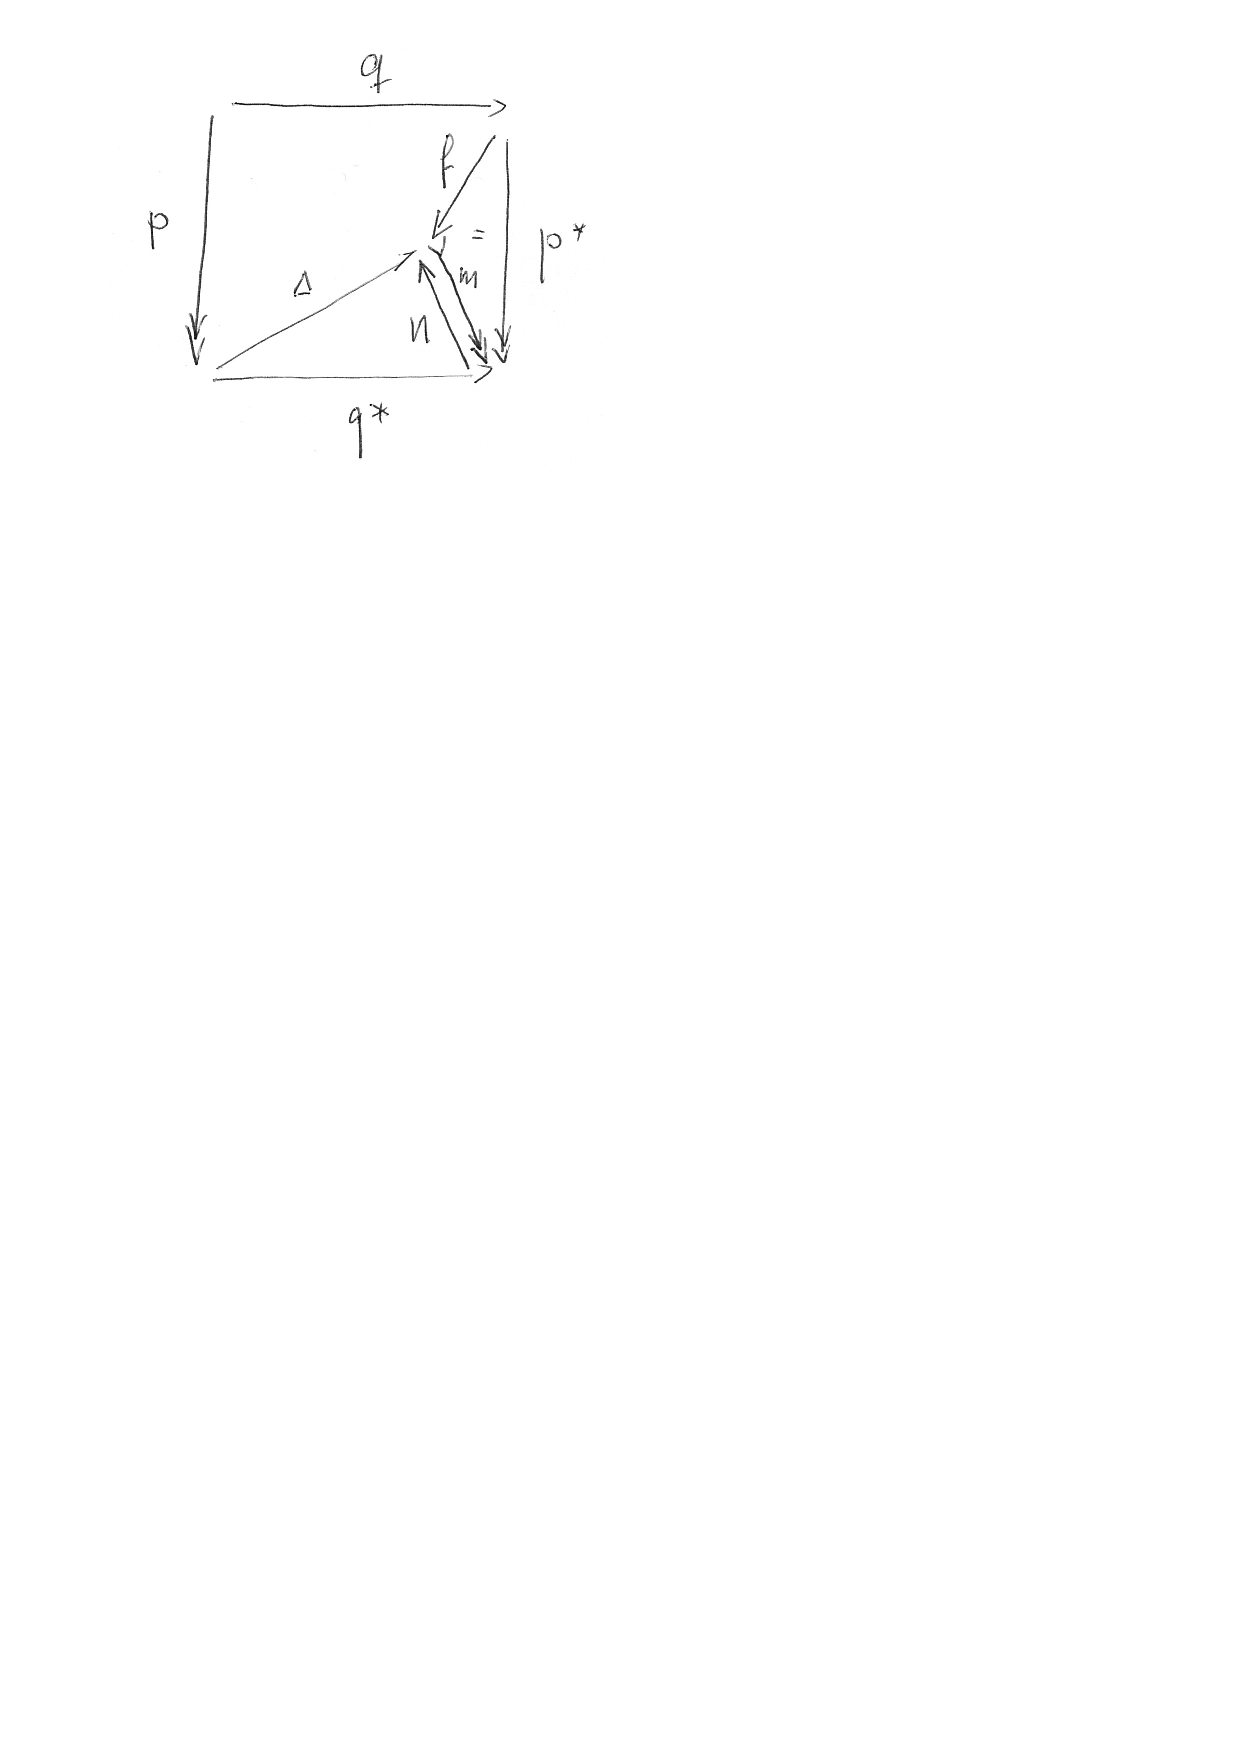
\includegraphics[width=0.22\textwidth]{Abbildungen/211}} \qquad \qquad \qquad
\subfigure[Pullback\label{fig:todo}]{
\includegraphics[width=0.22\textwidth]{Abbildungen/todo}}
\caption{Pushouts und Pullbacks}
\end{figure}

\begin{figure}[h]
\centering
\subfigure[Pushouts und extremal Epi\label{fig:212}]{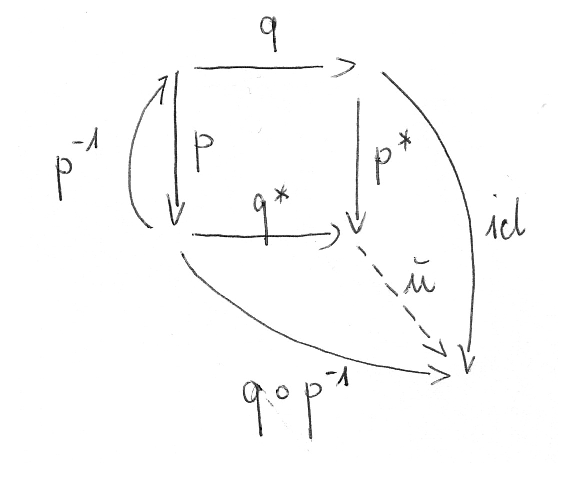
\includegraphics[width=0.22\textwidth]{Abbildungen/212}} \qquad \qquad \qquad
\subfigure[Pullback\label{fig:todo}]{
\includegraphics[width=0.22\textwidth]{Abbildungen/todo}}
\caption{Pushouts und Pullbacks}
\end{figure}
\newpage 

\begin{multicols}{2}
\columnseprule1pt

\textbf{\underline{Pushout}} 

\textbf{\coro 214 Pushouts bewahren Isomorphismen} \\
$(p^*, q^*)$ ist Pushout von $(p,q)$ und $p$ Iso $\implies$ $p^*$ ist Iso.

\textbf{\prop 215 Spezielle Pushouts in $Sys(\Sigma)$} \\
Wenn $(p:A\rightarrowtail B,q:A\rightarrowtail C)$ span extremaler Monos  in $\mathsf{Sys}(\Sigma)$, kann der pushout $(p^{*}:C\rightarrowtail D,q^{*}:B\rightarrowtail D)$
wie folgt konstruiert werden. Obda. Angenommen, dass $A_{s}$, $B_{s}$, und $C_{s}$ paarweise disjunkt sind, jede Sorte  $s$:

\begin{align*}
\textrm{\emph{(i)} } & \forall \, s\in S: \\ & D_{s}=A_{s}\cup\left(B_{s}-p(A_{s})\right)\cup\left(C_{s}-q(A_{s})\right)\\
\textrm{\emph{(ii)} } & \forall \, s \in S\textrm{ and }c\in C_{s}: \\ &  p_{s}^{*}(c)=\begin{cases}
a & c=q(a)\\
c & \textrm{otherwise} 
\end{cases}\\
\textrm{\emph{(iii)} } &  \forall \, s\in S\textrm{ and }b\in B_{s}: \\ & q^{*}(b)=\begin{cases}
a & b=q(a)\\
b & \textrm{otherwise}
\end{cases}\\
\textrm{\emph{(iv)} } &  \forall \, f \in O_{w,v}:\\ & f^{D}(x)=\begin{cases}
\left(p^{*}\right)^{v}(y_{C}) \, \, \, \, \, \,  \, \,  f^{C}(x_{C})=y_{C}\\
\, \, \, \, \, \,  \, \, \, \, \, \, \, \,  \, \, \, \, \, \, \, \,  \, \, \, \, \,  \textrm{ and }f^{C}(x_{C})=y_{C}\\
\left(q^{*}\right)^{v}(y_{B}) \, \, \, \, \, \,    \textrm{if }x=\left(q^{*}\right)^{w}(x_{B})\\
\, \, \, \, \, \,  \, \, \, \, \, \, \, \,  \, \, \, \, \, \, \, \,  \, \, \, \, \, \textrm{ and }f^{B}(x_{B})=y_{B}\\
\textrm{undefined} \, \, \, \, \, \,  \, \,  \textrm{otherwise}
\end{cases}
\end{align*}



\columnbreak

\textbf{\underline{Pullback}} 

\textbf{Weitere Pullbacks...} \\
Weitere siehe Skript.

\end{multicols}



\newpage

\section{Varietät}

\subsection{Atomare Axiome}

\paragraph{\defi 238 Atomares Axiom und Lösung}
Gegeben: $\Sigma = (S,O)$, atomares Axiom $a = (X, f)$ besteht aus einer endlichen Variablenmenge $X$ und einer Formel $f \in F^{\Sigma, X}$. \\
Eine Variablenzuweisung $h: X \rightarrow B$ in ein $\Sigma$-System B löst das Axiom $A = (X, f)$, wenn es einen \homo $h^*: \mathbf{A}_a \rightarrow B$ gibt, so dass $h^* \circ x^a = h$. \\
Wenn $h$ eine Lösung ist, schreiben wir $h \models a$

\paragraph{\prop 239 Homomorphismus und Lösung}

$h: X \nach B$ ist Lösung von atomarem Axiom $a = (X,f)$ in $B$ und $k: B \rightarrow C$ ist ein \homo $\implies k \circ h$ löst $a$ in $C$, d.h. $k \circ h \models a$.


\paragraph{\defi 240 Gültigkeit atomarer Axiome}

$a= (X,f) $ ist gültig in einem algebraischen System $B$ ($B \models a$), wenn jede Variablenzuweisung $h: X \nach B$ $a$ löst, d.h. \\
$B \models a$ wenn $\forall \, h: X \nach B :: h \models a$.

\paragraph{\prop 241 Gültigkeit ist abstrakt}
Wenn $a$ atomares Axiom ist, $B \models a$, und $B \approx B' \implies B' \models a$.  

\paragraph{\defi 242 Gefülltes algebraisches System}
Ein  algebraisches System $B$ ist gefüllt, wenn jede Trägermenge von $B$ nicht leer ist (d.h. 
$B_s \neq \emptyset$ für alle $s \in S$) \\ $S' \subseteq S \implies$ $B$ ist '$S'$-gefüllt', wenn $B_{s} \neq \emptyset \,$ für alle $s \in S'$.  

\paragraph{\prop 244 Gültigkeit in Produkten}
$a$ atomres Axiom, $I$ indizierte Menge. \\$(B_i \models a)_{i \in I} \implies \Pi(B_i)_{i \in I} \models a$


\paragraph{\prop 245 Gültigkeit in extremalen Subsystem}
$a$ atomares Axiom, $i: C \rightarrowtail B$ extremaler Mono, $B \models a \implies C \models a$

\emph{Notiz CT aus der Vorlesung: Wenn $C \models a$ und $h: B \rightarrowtail C$ injektiver Homo $\implies$: $B \models a$}

\paragraph{\defi 246: Homomorphe Bilder }
Algebraisches System $C$ ist homomorphes Bild eines Systems $B$, wenn es einen surjektiven Homomorphismus $q: B \twoheadrightarrow C$ gibt.

\emph{(Notiz: Homomorphes Bild ist Spezialfall von Epi (Vgl. Prop 80) (Bedenke: Wenn surjektiv, dann Epi. Umgekehrt nicht)) }


\paragraph{\prop 247: Gültigkeit in homomorphen Bildern}
$B \models a$, $C$ homomorphes Bild von $B$, d.h. Es gibt einen surjektiven \homo $q: B \twoheadrightarrow C \implies C \models a$



\paragraph{\coro 248: Gültigkeit in Produktkomponenten}
$a = (X,f)$ atomares Axiom und $S_X \subseteq S$ (Teilmenge der Sorten für welche $a$ Variablen hat), d.h. $s \in S_X \Leftrightarrow X_s \neq \emptyset$.
$\Pi (B_i)_{i \in I} \models a$ und $(B_{i,s} \neq \emptyset)_{i \in I, s \in S_X}$ ('$S_X$' gefüllt) \\
$\implies  B_i \models a \, \, \forall \,  i \in I $ (jede Komponente des Produktes erfüllt das Axiom).

\paragraph{\lem 249: Variablenzuweisung in approximierte Systeme}
(ausgelassen)

\paragraph{\prop 250: Gültigkeit in approximierte Systemen}
(ausgelassen)


\subsection{Atomare Spezifikationen}

\paragraph{\defi 251: Atomare Spezifikation, Varietäten} 
Atomare Spezifikation \\ $ASpec = (\Sigma, \Phi)$ besteht aus einer Signatur $\Sigma$ und einer Menge von atomaren Axiomen $\Phi$ wrt. $\Sigma$.
$B \in Sys(\Sigma) $ erfüllt die Spezifikation (geschrieben: $B \models ASpec$), wenn $B \models a$ für alle $a \in \Phi$. \\
Die volle Subkategorie von \syssig, welches alle Systeme beinhaltet, die die Spezifikation $ASpec = (\Sigma, \Phi)$ erfüllen, wird bezeichnet als Sys($ASpec$) oder Sys$(\Phi)$. \\
Eine volle Subkategorie $\mathbb{K}$ aller $\Sigma$-Systeme wird eine Varietät genannt, wenn es eine atomare Spezifikation ($\Sigma, \Phi$) gibt, so dass $\mathbb{K} = Sys(\Phi)$


\paragraph{\prop 252: Varietäten sind abstrakt} 
Jede Varietät ist isomorph-geschlossen.

\paragraph{\defi 253: Bündel atomarer Axiome, Lösungen} 
Ein Bündel $\mathcal{B}$ atomarer Axiome mit den selben Variablenmengen $X$ ist eine syntaktische Präsentation $\mathcal{B} = (X, F \subseteq F^{\Sigma, X})$.
$C$ erfüllt ein Bündel (geschrieben: $C \models \mathcal{B}$), wenn jede Variablenzuweisung $h: X \nach C$ erweitert werden kann auf einen \homo $h^*: \mathbf{A}_\mathcal{B} \nach C$, so dass $h^* \circ^\mathcal{B} = h$


\paragraph{\lem 254: Bündel definieren Co-Limiten} 
(ausgelassen)

\paragraph{\prop 255: Bündel atomarer Axiome} 

$(a_i)_{i \in I}$ ist Familie atomarer Axiome mit den selben Variablenmengen $X$, d.h. $a_i = (X, f_i)$ für alle $i \in I$ \\ 
$\implies C $ erfüllt alle Axiome $((C \models a_i )_{i \in I})$ $\Leftrightarrow$ $C$ erfüllt das Bündel $\mathcal{B} = (X, \{f_i:: i \in I \})$, d.h. $C \models \mathcal{B}$ 

\paragraph{\lem 256: Co-well-powered Basis} 
\syssig its co-well-powered.


\paragraph{\coro 257: Varietäten sind episch-reflektive Subkategorien}
Jede Varietät $\mathbb{K} \subseteq Sys(\Sigma)$ ist episch-reflektive Subkategorie von \syssig.

\paragraph{Theorem 258: Birkhoffs Charakterisierung}
Eine volle Unterkategorie $\mathbb{K}$ von \syssig ist eine Varietät $\Leftrightarrow $ $\mathbb{K}$ ist geschlossen bis auf Produkte, extremale Subobjekte, homomorphe Bilder und approximierte Systeme. 
 
 
\newpage  
\subsection{Spezifikationsproblem und einfache Lösung}

\paragraph{\defi 259: Spezifikationsproblem, einfache Lösung}
Ein Spezifikationsproblem ist gegeben durch eine Signatur $\Sigma$ und entweder 
\begin{enumerate}
\item Ein $\Sigma$-System K oder
\item Eine volle und isomorph-geschlossene Subkategorie $\mathbb{K} \subseteq Sys(\Sigma)$ 
\end{enumerate}
Eine einfache Lösung für das Spezifikationsproblem ist eine atomare Spezifikation $ASpec = (\Sigma, \Phi)$, so dass 
\begin{enumerate}
\item $K$ ist initial in $Sys(ASpec)$ oder
\item $Sys(ASpec) = \mathbb{K}$
\end{enumerate}


\paragraph{\coro 261: Reflektion des initialen Objektes}
$\mathcal{D}$ relflektive Subkategorie von $\mathcal{C}$, $\mathcal{C}$ hat initiales Objekt $\mathcal{I}$ $\implies$ Reflektion $\mathcal{I}_{\mathcal{D}}$ von $\mathcal{I}$ ist initial in $\mathcal{D}$

\paragraph{\coro 262: Spezifizierbare Systeme}
Eine Spezifikationsproblem $K \in Sys(\Sigma)$ vom Typ 1. (siehe Defi 259 1.) ist lösbar $\Leftrightarrow$ $K$ ist generiert durch seine Operationen, d.h. $K = \left\lceil i\left(\emptyset^{\Sigma}\right)\right\rceil ^{c}$, wobei $i: \emptyset^\Sigma \rightarrow K$ ist der eindeutige Homomorphismus vom initialen Objekt nach $K$.

\section{Quasi Varietäten}

\subsection{Horn-Typ Axiome}

\paragraph{\defi 264: Hornaxiom}
Hornaxiom $a = (X, P \subseteq F^{\Sigma,X}, c \in F^{\Sigma,X})$ \\
$X$ ist endliche Variablenmenge, $P$ (Prämisse) endliche syntaktische Präsentation, $c \in F^{\Sigma,X}$ Formel (Konklusion).

\paragraph{\defi 265: Gültigkeit von Hormaxiomen}
Hormaxiom $a = (X, P, c)$ ist gültig in einem algebraischen System $B$ $(B \models a)$, wenn jeder Morphismus \\ $h: \mathbf{A}_P \nach B$ erweitert werden kann zu einem \homo \\ $h^*: \mathbf{A}_{c^P} \nach B$, so dass $h^* \circ x_{p}^c = h$, wobei $c^p = (X,P \cup \{c\})$ und $x^{c}_P: \mathbf{A}_P \nach \mathbf{A}_{c^P}$ ist der eindeutige \homo, der $x_P^c \circ x^P = x^{c^P}$ erfüllt.

\paragraph{\prop 266: Gültigkeit ist abstrakt}
$a = (X, P, c)$ Hornaxiom, $B \models a$, $B \approx B'$ $\implies$ $B' \models a$.


\paragraph{\prop 267: Gültigkeit Produkt und Subsystem}
$a = (X, P, c)$ Hornaxiom
\begin{enumerate}
\item $I$ Indexmenge, $(B_i \models a)_{i \in I}$ $\implies$ $\Pi (B_i)_{i \in I} \models a$
\item $i: C \rightarrowtail B$ extremal Mono, $B \models a$ $\implies $ $C \models a$
\end{enumerate}

\paragraph{\lem 268: \homos in approximierte Systeme}
$(I, \leq)$ gerichtete Indexmenge $\mathcal{H} = \left( (B^I)_{I \in I} (k^{i,j}: B^i \nach B^j)_{i,j \in I, i \leq j} \right)$ approximierte Situation \\ mit approximierende System 
$\left(\mathcal{H}{}^{\bullet},\left(i^{\bullet}:B^{i}\rightarrow\mathcal{H}{}^{\bullet}\right)_{i\in I}\right)$,
\\ $F=\left(X,F\subseteq F^{\Sigma,X}\right)$ endliche syntaktische Präsentation, \\
 $m:\mathbf{A}_{F}\rightarrow\mathcal{H}{}^{\bullet}$ homo, \\
$\implies$ es gibt $j\in I$ und ein Homo $m':\mathbf{A}_{F}\rightarrow B^{j}$, so dass  $m=j^{\bullet}\circ m'$.


\paragraph{\prop 269: Gültigkeit in  approximierten Systeme}
$(I, \leq)$ ist eine gerichtete, partiell geordnete Indexmenge und $\mathcal{H} = \left( (B^i)_{i \in I}, (k^{i,j}: B^i \nach B^j)_{i,j \in I, i \leq j} \right)$ eine approximierende Situation, so dass $(B^i \models a)_{i \in I}$ für ein Hornaxiom $a$ \\
$\implies $ $a$ ist gültig im approximierten System $\mathcal{H}^\bullet$, d.h. $\mathcal{H}^\bullet \models a$

\subsection{Horntyp Spezifikation}

\paragraph{\defi 270: Horn-Spezifikation}
Ein Horntyp-Spezifikation $HSpec = (\Sigma, \Phi)$ besteht aus einer Signatur $\Sigma$ und einer Menge an Hornaxiomen $\Phi$ wrt. to $\Sigma$. \\
Algebraisches System $B \in Sys(\Sigma)$ erfüllt die Spezifikation $(B \models HSpec$  oder $B \models \Phi)$, wenn $B \models a$ für alle $a \in \Phi$.  \\
Die volle Subkategorie von $Sys(\Sigma)$, welche alle Systeme beinhaltet, die die Spezifikation $HSpec = (\Sigma, \Phi)$ 
erfüllen, wird bezeichnet als $Sys(HSpec)$ oder $Sys(\Phi)$. \\
Eine volle Subkategorie $\mathbb{K}$ aller $\Sigma$-Systeme wird Hornklasse genannt, wenn es eine Hornspezifikation $HSpec = (\Sigma, \Phi)$ gibt, so dass $\mathbb{K} = Sys(HSpec)$.

\paragraph{\prop 271: Hornklassen sind abstrakt}
Jede Hornklasse ist isomorph-geschlossen.

\paragraph{\defi 272: Bündel von Hornaxiomen, Lösung}
Ein \emph{Bündel }$\mathcal{B}=\left(X,P\subseteq F^{\Sigma,X},C\subseteq F^{\Sigma,X}\right)$\emph{
von Hormaxiomen} mit der gleichen endlichen Variablenmenge  $X$ \emph{und}
der gleichen endlichen Menge  von prämissen $P$ besteht aus zwei syntaktischen Präsentationen
$P$ und $C$. \\
Die syntaktische Präsentation für Prämisse und Konklusion wird bezeichnet als $C^{P}=(X,P\cup C)$. \\
Der eindeutige Epimorphismus, der $x_{P}^{C}\circ x^{P}=x^{C^{P}}$ erfüllt, wird bezeichnet als  $x_{P}^{C}:\mathbf{A}_{P}\rightarrow\mathbf{A}_{C^{P}}$. \\
Ein algebraisches System $D$ erfüllt ein Bündel  ($D\models\mathcal{B}$),
wenn jeder Homo $h:\mathbf{A}_{P}\rightarrow D$ erweitert werden kann
zu einem Homo $h^{*}:\mathbf{A}_{C^{P}}\rightarrow C$, so dass
$h^{*}\circ x_{P}^{C}=h$.

\paragraph{\lem 273: Bündel definieren Co-Limiten}
$\left(a_{i}=\left(X,P,c_{i}\right)\right)_{i\in I}$ ist eine Familie von Hornaxiomen, mit der selben Variablenmenge
$X$ und der selben Menge von Prämissen $P$ und dessen Bündel $\mathcal{B}$ \\ 
$\implies$  $\mathbf{A}_{\mathcal{B}}$
ist Co-Limit von $\left(x^{c_{i}^{P}}:\mathbf{A}_{P}\rightarrow\mathbf{A}_{c_{i}^{P}}\right)_{i\in I}$

\paragraph{\lem 274: Bündel von Hornaxiomen}
Wenn $(a_i)_{i \in I}$ ist Familie von Hornaxiomen mit der gleichen Variablenmenge $X$ und der gleichen Menge von Prämissen, das heißt $a_i = (X, P, c_i)$ für alle $i \in I$ \\
dann $\implies$ ein algebraisches System $D$ erfüllt alle Axiome, d.h. $(D \models a_i)_{i \in I}$ $\Leftrightarrow$ $D$ erfüllt das Bündel $\mathcal{B} = (X, P, \{c_i:: i \in I\})$, d.h. $D \models \mathcal{B}$

\paragraph{Theorem 276: Charakterisierung von Hornklassen}
Eine volle Subkategorie $\mathbb{K}$ von $Sys(\Sigma)$ ist eine Hornklasse $\Leftrightarrow$ $\mathbb{K}$ ist geschlossen bis auf Produkte, extremale Subobjekte und approximierte Systeme.





\end{document}